\documentclass[11pt,a4paper]{article}

\usepackage[polish]{babel}
\usepackage{polski}
\usepackage[utf8]{inputenc}
\usepackage[T1]{fontenc}
\usepackage[pdftex]{graphicx}
\usepackage{color}
\usepackage{placeins}
\usepackage[math]{anttor}
\usepackage{natbib}
\usepackage{url}
\usepackage{float}
\usepackage[font=footnotesize,labelfont=bf,justification=centering]{caption}
\usepackage{array}
\frenchspacing

\newcommand{\HRule}{\rule{\linewidth}{0.5mm}}

\newcommand{\todo}[1]{\colorbox{yellow}{#1}}

\begin{document}

\begin{titlepage}

\begin{center}
\includegraphics[width=2cm]{gfx/agh-logo.png}\\[1cm]

\textsc{\LARGE Akademia Górniczo-Hutnicza\\im. Stanisława Staszica w Krakowie}\\[0.5cm]
\textsc{\Large Wydział Elektrotechniki, Automatyki, Informatyki i Elektroniki}\\[0.5cm]
\textsc{\Large Katedra Informatyki}\\[1.5cm]
\textsc{\Large Praca magisterska}\\[0.5cm]

\HRule \\[0.4cm]
{ \Large \bfseries Automatyczna klasyfikacja i ekstrakcja tematu krótkich wiadomości tekstowych w języku polskim}\\[0.4cm]

\HRule \\[1.5cm]
\begin{minipage}{0.4\textwidth}
\begin{flushleft} \large
\emph{Autor:}\\
Paweł Obrok
\end{flushleft}
\end{minipage}
\begin{minipage}{0.4\textwidth}
\begin{flushright} \large
\emph{Promotor:} \\
dr inż. Michał Korzycki
\end{flushright}
\end{minipage}

\vfill

{\large Kraków 2012}

\end{center}

\end{titlepage}

\begin{center}
\vfill

\textsc{\Large Oświadczenie autora}\\[0.5cm]
\textsc{Oświadczam, świadomy odpowiedzialności karnej za poświadczenie nieprawdy, że niniejszą pracę dyplomową wykonałem osobiście i samodzielnie i że nie korzystałem ze źródeł innych niż wymienione w pracy.}\\[0.5cm]
\end{center}
\pagebreak

\tableofcontents
\pagebreak

\section{Wstęp}

Poniższy rozdział przybliża temtykę pracy oraz opisuje jej zawartość.

\subsection{Wprowadzenie}

Metody automatycznego przetwarzania tekstu nabierają w dzisiejszym świecie
coraz większego znaczenia --- jesteśmy zalewani przez powodź informacji, a
większość z nich ma właśnie postać tekstową. Aby poradzić sobie z tym ogromem
napływających bodźców próbujemy uciekać się do mechanizmów, które pozwolą je
przeanalizować albo przynajmniej wstępnie przetowrzyć. Technologie w rodzaju
wyszukiwarek internetowych, agregatorów wiadomości czy baz filmów lub książek
potrafiących wskazać dzieła podobne do tych, które nam się podobały stają się
coraz popularniejsze i często koniecznie do znalezienia pożądanej informacji.

Wspomniane mechanizmy zajmują się głównie segregowaniem czy przeszukiwaniem
danych, ale wyobrażalne są również zadania na wyższym poziomie koncepcyjnym.
Chcielibyśmy, aby odpowiednio zaprogramowane maszyny były w stanie rozumieć
tekst tak jak ludzie i przetwarzać go nie tyle jako ciągi znaków ile jako idee,
opisy zdarzeń itp. wyrażone tymi znakami. Zadania takie jak automatyczne
tłumaczenie, generowanie streszczeń lub parafrazowanie tekstów wydają się na
tym etapie wymagać takiego właśnie zrozumienia i nadal ich sprawne wykonywanie
pozostaje wyłączną domeną człowieka mimo postępujących prac w tych
dziedzinach.

Naczelnym problemem, który należy przezwyciężyć w tego typu zagadnieniach jest
fakt, że słowo pisane, a ogólniej język odnoszą się do pewnej rzeczywistości
zewnętrznej, a wręcz jest to ich zasadniczą funkcją. Maszyny, które
przetwarzają tekst nie mają zwykle bezpośredniej styczności z tą
rzeczywistością, starając się operować jedynie na ciągach symboli. Ujawnia się
tutaj przewaga w tym polu ludzi, którzy mają wiele lat na zbieranie informacji
o świecie i o tym w jaki sposób odnosi się do niego język, którym się
posługują.

Istnieje wiele kierunków badań mających rzucić więcej światła na rozwiązanie
tego problemu. Najbardziaj ambitne zakładają, że konieczne jest tutaj
stworzenie uniwersalnej sztucznej inteligencji, czyli maszyny o możliwościach
podobnych ludzkiemu umysłowi, która miałaby dostęp do bodźców zmysłowych
dokładnie tak jak człowiek i byłaby w jakimś sensie w stanie rozumieć
język i rzeczywistość, którą opisuje.

Nieco mniej radykalne podejście sugeruje budowę ontologii, czyli
sformalizowanego opisu znaczeń wyrazów i powiązań między nimi wraz z typami
tych powiązań. Przykładowo mogłaby ona zawierać wpis ,,tryb part-of zegar''
reprezentujący fakt, że zegary często zawierają tryby jako części. Taka baza
wiedzy opisuje znaczenie słów niejako przez przykłady kontekstów, w których
mogą występować i pozwala dokonywać rozumowania na temat tekstu w rodzaju
wykrywania synekdochy (wykorzystywania całości na oznaczenie części lub
odwrotnie, np. ,,Hollywood'' zamiast ,,Amerykański przemysł filmowy''), co
umożliwi odkrycie jego prawdziwego znaczenia.

Jeszcze inne podejście, któremy poświęcona jest ta praca, polega na próbie
wykrywania powiązań w samym analizowanym tekście. U jej podstaw leży
obserwacja, że wyrazy będą pojawiać się częściej w kontekście wyrazów
związanych z nimi znaczeniowo, przykładowo ,,żaba'' może pojawić się blisko
,,skakać'' czy ,,pływać'', rzadziej ,,biegać''. Znów daje nam to zestaw
kontekstów dla danego wyrazu, tym razem jednak należy go wyekstrahować z
tekstu, a częściej zbioru tekstów, natomiast konteksty dla słów, które w takim
korpusie się nie pojawią, nie są w ogóle dostępne. Metody tego rodzaju mają
jednak tę zaletę, że operują jedynie na tekście, nie potrzebują dodatkowych
informacji w przeciwieństwie do przedstawionych wyżej podejść.

Najprostszą wersją tego podejścia jest Vector Space Modelling - metoda
polegająca na reprezentowaniu dokumentów jako wektorów, których współrzędne
odpowiadają w jakiś sposób częstościom występowania w nich pewnych wyrazów.
Pozwala to na porównywanie dokumentów metodami algebry liniowej, na przykład
ocenianie podobieństwa dokumentów przez pomiar kąta między odpowiadającymi im
wektorami.

VSM wykazuje niestety znaczne wady, przykładowo jest całkowicie nieczułe na
istnienie synonimów albo możliwość występowania słowa w więcej niż jednym
znaczeniu. Co więcej duża część wyrazów w dokumentach to z semantycznego
punktu widzenia szum, przykładowo znaki przestankowe, chociaż występują dość
często nie są zwykle kluczowe do zrozumienia tekstu. Aby uporać się z tymi
wadami proponuje się różne udoskonalenia tej metody. Ta praca zajmuje się
porównaniem dwóch z nich --- Latent Semantic Indexing oraz Latent Dirichlet
Analysis.

LSI to metoda pochodząca wprost z algebry liniowej. Sprowadza się ona do
wprowadzenia nowej, mniejszej bazy do przestrzeni wektorów odpowiadających
dokumentom w taki jednak sposób, aby zachować jak najwięcej informacji
zawartych w oryginalnej reprezentacji. Ma to wyeliminować szum, a także wykryć
związki między wyrazami przez ich wspólne występowanie w wektorach nowej bazy.

LDA stawia sobie za cel przedstawienie przynajmniej częściowego
probabilistycznego modelu powstawania dokumentów i założywszy poprawność tego
modelu znalezienie jego parametrów dla danego korpusu. Ze względu na specyfikę
tego modelu, konkretnie założenie o tym, że na każdy tekst składa się jeden lub
więcej tematów i pojawienie się w nim każdego wyrazu można przypisać jednemu z
tych tematów, również pozwala on wykrywać zależności między słowami. W tym
wypadku zależności te będą zadane przez występowanie słów w tym samym temacie.

Zarówno LSI jak i LDA mogą być wykorzystane w szeregu zastosowań związanych z
automatycznym przetwarzaniem tekstu, takich jak wyszukiwanie dokumentów w
korpusie, automatyczna ekstrakcja słów kluczowych czy ocena podobieństwa
dokumentów. Praca ta stawia sobie za zadanie porównanie działania tych metod
w tego typu zadaniach.

Istnieją już porównania LSI i LDA, jak choćby \cite{lda-paper}, jednak traktują
one głównie o języku angielskim, który ma względnie prostą fleksję. Wyniki te
nie zawsze przenoszą się na inne języki, jak choćby polski --- wykorzystany do
testów w tej pracy --- gdzie każdy wyraz występuje w bardzo wielu formach. Aby
rozwiązać ten problem zastosowano wraz z metodami LSI i LDA słownik fleksyjny
języka polskiego - \cite{lubaszewski-slownik}. Poddano także porównaniu wyniki
osiągane z i bez jego zastosowania.

\subsection{Zawartość pracy}

Rozdział \ref{sec:theory} poświęcony jest teoretycznemu opisowi porównywanych
metod, jak i metryk stosowanych do ich oceny. W rozdziale \ref{sec:data} opisany
został zbiór danych użytych do testów i wygenerowany przy jego użyciu testowy
problem, natomiast w rozdziale \ref{sec:solution} opisane są mechanizmy użyte
do jego rozwiązania. Rozdział \ref{sec:results} zawiera uzyskane wyniki
numeryczne wraz z ich omówieniem, a rozdział \ref{sec:summary} podsumowuje
pracę i proponuje dalsze ścieżki jej rozwoju.

Dodatek \ref{sec:terms} omawia najczęściej pojawiające się w tej pracy
terminy i oznaczenia.  Ponadto w dodatku \ref{sec:code} podano sposób
wykorzystania kodu użytego do uzyskania wyników przedtstawionych w tej pracy. W
dodatku \ref{sec:full-results} zawarto pełną tabelę tematów wygenerowanych
dla przykładowych danych.

\pagebreak


\section{Podstawy teoretyczne}
\label{sec:theory}

W tym rozdziale opisana jest ogólnie koncepcja wektorowego modelowania
dokumentów oraz metody, które poddano porównaniu w tej pracy, a które od tej
koncepcji pochodzą. W dalszej części rozdziału zawarto opis metryk perpexity,
dokładności i kompletności wykorzystywanych przy ocenie działania modeli
językowych i systemów wyszukiwania informacji.

\subsection{Vector Space Model}

Model przestrzeni wektorowej (Vector Space Model --- VSM) to metoda modelowania
języka polegająca na reprezentowaniu dokumentów jako wektorów co umożliwia na
przykład porównywanie ich metodami algebry liniowej.  Wektor dla $i$-tego
dokumentu ma postać:

\begin{equation}
d_i = (w^i_0, w^i_1, \ldots, w^i_N)
\end{equation}

\noindent
gdzie wymiar $w^i_k$ odpowiada $k$-temu tokenowi ze słownika. Współczynniki te
nazywane są także wagami i mają oddawać znaczenie danego tokenu w danym
dokumencie --- powinny być tym wyższe, im bardziej kluczowy dla sensu $i$-tego
dokumentu jest $k$-ty token. Przyjmuje się zwykle, że wymiary odpowiadające
tokenom nie występującym w danym dokumencie są zerowe.

\subsubsection{Schemat wagowy}
\label{weighting-theory}
Najbardziej ogólnie wagi $w^i_k$ uzyskuje się przez pomnożenie wagi globalnej
$g_k$, która ma odzwierciedlać popularność tokenu w całym korpusie i wagi
lokalnej $l^i_k$, która opisuje stricte znaczenie tokenu w danym dokumencie.
Tabele \ref{global-weights} i \ref{local-weights} podsumowują popularnie
stosowane wagi globalne i lokalne. Ich drobiazgowe porównanie dla języka
polskiego znaleźć można w \cite{figiel}. Dobór tych dwóch wag nazywamy
schematem wagowym.

\begin{table}[h]
\caption{Możliwe wagi globalne $g_k$}
\label{global-weights}
\begin{tabular}[c]{|c|p{0.7\linewidth}|}
\hline
$1$ & Brak wagi globalnej --- częstość występowania tokenów w całym korpusie jest ignorowana \\\hline
$\frac{1}{\sum_j (l^j_k)^2}$ & Normalizacja --- tutaj przez sumę kwadratów wag lokalnych tokenu w całym korpusie\\\hline
$\frac{gf_k}{df_k}$ & gf-idf --- waga tym większa, im więcej razy występuje dany token i tym mniejsza, im więcej dokumentów go zawiera\\\hline
$log(\frac{n}{df_k}) + 1$ & idf --- logarytm z liczby dokumentów w których występuje dany token znormalizowanej przez liczbę wszystkich dokumentów\\\hline
$1 - \sum_{i/0}^n \frac{tf^i_klog(tf^i_k)}{log(n)}$ & Entropia --- waga pochodząca z teorii informacji, ilość informacji którą daje pojawienie się danego tokenu o numerze tekstu, w którym to nastąpiło\\\hline
\end{tabular}
\end{table}

\begin{table}[h]
\caption{Możliwe wagi lokalne $l^i_k$}
\label{local-weights}
\begin{tabular}[c]{|c|p{0.875\linewidth}|}
\hline
$1$ & Waga binarna --- zachowana zostaje jedynie informacja o fakcie wystąpienia tokenu, liczba wystąpień jest ignorowana\\\hline
$t^i_k$ & Częstość występowania --- najprostsza waga, można powiedzieć, że inne są próbą jej usprawnienia przez odpowiednie wygładzenie\\\hline
$\sqrt{t^i_k}$ & Wygładzona częstość występowania --- aby oddać fakt, że kolejne wystąpienia tego samego wyrazu dają stosunkowo mniejszą wskazówkę co do jego znaczenia dla danego dokumentu, można wygładzić częstość występowania pierwiatskiem lub logarytmem\\\hline
\end{tabular}
\end{table}

Konkretny schemat wagowy dobiera się empirycznie, często pod jakąś klasę
problemów. Dla zadań typu information retrieval dobrze sprawdzają się lokalne
wagi wygładzone i entropia jako waga globalna, z czego można wywnioskować, że
obserwacja o mniejszym znaczeniu kolejnych wystąpień tokenu w tym samym
dokumencie jest trafna.

Brak wagi globalnej daje z reguły znacznie gorsze wyniki niż pozostałe
możliwości. Jej zastosowanie pozwala automatycznie wykryć wyrazy takie jak
spójniki, które występują bardzo często we wszystkich tekstach, a nie mają
dużego ładunku semantycznego. W korpusach dotyczących jednej dziedziny mogą się
pojawić inne wyrazy o takiej charakterystyce, przykładowo wyraz ,,wyraz''
występuje bardzo często w tej pracy i najprawdopodobniej nie niesie wiele
informacji o tematyce poszczególnych jej akapitów, w których się pojawia.

Podobnie zastosowanie binarnej wagi lokalnej negatywnie wpływa na jakość
otrzymywanych wyników. Utrata informacji na temat dokumentu jest w tym wypadku
zbyt duża, dodatkowe wystąpienia tokenu, mimo iż nie tak znaczące jak pierwsze,
są jednak wskazówką co do większego znaczenia tego tokenu w tekście.

\subsubsection{Podobieństwo dokumentów}

Aby ocenić podobieństwo dwóch dokumentów w modelu przestrzeni wektorowej
stosuje się miarę kosinusową --- kosinus kąta między wektorami reprezentującymi
te dokumnety. Dla wektorów dokumentów $d^i$ i $d^j$ wynosić ona będzie:

\begin{equation}
  d(d^i, d^j) = \langle \frac{d_i}{||d^i||}, \frac{d^j}{||d^j} \rangle
\end{equation}

\noindent
gdzie $\langle \bullet, \bullet \rangle$ oznacza iloczyn skalarny, a $||d|| =
\lbrace d, d \rbrace$. Daje to liczbę z przedziału $[-1,1]$, gdzie $-1$ oznacza
dokumenty skrajnie różne, a większe wartości coraz większe podobieństwo.
Wartość $1$ osiągnięta zostanie dla dwóch dokumentów, w których względna
częstość występowania słów (ewentualnie znormalizowana) jest taka sama.

\subsubsection{Wady}

Zgodnie z przedstawionym mechanizmem działania wszystkie wyrazy, które mają
różne postaci w zapisie, traktowane są jako całkowicie osobne wymiary
przestrzeni wektorowej. Pomijana jest także możliwość występowania wyrazów w
wielu formach (fleksja), możliwość oznaczenia tego samego pojęcia przez wiele
różnych ciągów symboli (synonimy) oraz możliwość, że dany ciąg symboli może
opisywać kilka różnych pojęć (polisemia).

Aby mitygować te niedociągnięcia stosowane są różne rozszerzenia modelu
przestrzeni wektorowej. Opisany w rozdziale \ref{sec:clp} słownik fleksyjny
pozwala sprowadzić wyrazy do formy podstawowej, co ,,spłaszczy'' je na powrót w
jeden wymiar. Opisane w dalszych dwóch rozdziałach metody redukcji wymiarowości
macierzy pozwalają wyekstrahować najczęściej pojawiające się kombinacje
wyrazów i częściowo zredukować problem synonimów. Aby radzić sobie z polisemią
możliwe jest zastosowanie mechanizmów kontekstowego ujednoznaczniania wyrazów.

\FloatBarrier

\subsection{Latent Semantic Indexing}

Metoda LSI to rozszerzenie modelu przestrzeni wektorowej mające na celu
uzyskanie lepszych wyników dzięki automatycznej identyfikacji powiązań między
wyrazami występującymi w dokumencie przez redukcję wymiaru macierzy
term-dokument. Rozwiązuje to wspomniany wcześniej problem synonimów i do
pewnego stopnia polisemii.  Istnieje przy tym nadzieja, że przez odpowiednie
dobranie mechanizmu redukcji wymiaru macierzy usunięty zostanie szum, przy
jednoczesnym zachowaniu zawartej w niej informacji.

\subsubsection{Intuicja}

Dzięki temu, że traktujemy dokumenty jako elementy przestrzeni wektorowej,
możliwe staje się wprowadzenie dowolnej bazy w tej przestrzeni i
reprezentowanie wektorów przy jej użyciu. Jedną ze stosowanych do tego metod
jest SVD. SVD stara się znaleźć taką bazę przestrzeni, żeby jej kolejne
współrzędne posorotwane były w kolejności malejącej wariancji wektorów z danego
zbioru (w tym wypadku korpusu) w ich kierunku. Następnie po przeniesieniu
wektorów do tej bazy możliwe jest odcięcie współrzędnych dalszych niż $n$-ta
przy utracie minimalnej ilości informacji.

W przypadku zastosowania SVD do przestrzeni dokumentów wektory nowej bazy można
traktować właśnie jako tematy dokumentów z korpusu. Każdy z nich będzie
opisywał kierunek w starej przestrzeni, wzdłuż którego dokumenty są jak
najbardziej różne, a przez to wskazuje on na powiązanie między swoimi
składowymi przez ich skorelowanie z tą właśnie różnicą.

\subsubsection{Singular Value Decomposition}

SVD to sposób rozkładu macierzy na iloczyn macierzy o pewnych szczególnych
własnościach, które okazują się przydatne w zastosowaniach związanych na
przykład z przetwarzaniem sygnałów. Każdą macierz $M$ o wartościach będących
liczbami zespolonymi można przedstawić jako:

\begin{equation}
  \label{svd}
  M = U\Sigma V^*
\end{equation}

\noindent
Przy czym macierz $\Sigma$ jest macierzą diagonalną, która na przekątnej
zawiera wartości osobliwe macierzy $M$, macierz $U$ zawiera lewe wektory
osobliwe $M$, a macierz $V^*$ jest macierzą sprzężoną do macierzy zawierającej
prawe wektory osobliwe $M$.

Tak zdefiniowany rozkład pozwala na redukcję rzędu macierzy zgodnie z
twierdzeniem Eckharta-Younga, które głosi, że macierz o rzędzie $k$, najlepiej
przybliżająca $M$ w sensie normy Frobeniusa czyli pierwiastka sumy kwadratów
różnic odpowiadających sobie elementów macierzy jest zadana przez:

\begin{equation}
  M \approx \tilde{M} = U\tilde{\Sigma} V^*
\end{equation}

\noindent
Gdzie macierz $\tilde{\Sigma}$ uzyskuje się poprzez wybranie $k$ największych
wartości osobliwych i zastąpienie pozostałych zerami w macierzy $\Sigma$.

\subsection{Latent Dirichlet Allocation}
\label{sec:lda}

Podczas gdy LSI ma u swoich podstaw metodę algebraiczną redukcji wymiarowości
macierzy przy utracie jak najmniejszej ilości zawartej w tej macierzy
informacji, intuicja stojąca za LDA jest znacznie bliżej spokrewniona z
wyobrażeniami na temat powstawania dokumentów tekstowych. Jak zostanie jednak
przedstawione w tym rozdziale, ostatecznie LDA również sprowadza się do redukcji
wymiaru macierzy term-dokument przez wprowadzenie nowej przestrzeni, w której
reprezentowane będą dokumenty.

Metoda LDA została zaproponowana przez Davida Blei et al. w 2003 roku w
\cite{lda-paper}.

\subsubsection{Intuicja}

LDA to probabilistyczny model generatywny opisujący powstawanie dokumentów.
Zakłada, że dokumenty są zbiorami wyrazów i kolejność ich występowania nie ma
znaczenia (założenie bag-of-words). Zakłada następnie, że każdy dokument
traktuje o małej liczbie tematów z pewnego zbioru tematów, których liczba jest
znana \emph{a priori}.

Proces generowania dokumentów przebiega przez powtarzanie dwuetapowego
losowania: najpierw z dystrybucji tematów dla danego dokumentu losowany jest
temat, a następnie z dystrybucji wyrazów w tym temacie losowany jest kolejny
wyraz.

\subsubsection{Budowa modelu}

Mechanizm Latent Dirichlet Allocation opiera się na założeniu, że dany dokument
bądź wyraz związany jest z pewną liczbą tematów.  Model dla Latent Dirichlet
Allocation jest macierzą $K \times V$ (dla $K$: liczba tematów, $V$ -
rozmiaru słownika) gdzie wiersz oznacza prawdopodobieństwo  przynależności
danego wyrazu do danego tematu.  Rozkład tematów dla danych dokumentów i
wyrazów jest modelowy przez rozkład Dirichleta, którego parametry są estymowane
na podstawie obserwowanego korpusu. Rozkład Dirichleta jest faktycznie rodziną
ciągłych rozkładów wielu zmiennych parametryzowaną przez wektor $\alpha$
dodatnich parametrów rzeczywistych (stanowi wielowymiarowe uogólnienie rozkładu
beta).  Algorytm zastosowany tu do estymacji modelu to online variational Bayes
algorithm for Latent Dirichlet Allocation \cite{gensim-algorithm}.

\subsection{Perplexity}

Współczynnik perplexity, który zaproponowany został do oceny modeli języka
\cite{bahl-perplexity}, ma oddawać niejako poziom ''zaskoczenia'' niewidzianymi
dotąd danymi. Dla rozkładu prawdopodobieństwa $p$ definiujemy go jako
eksponentę entropii $p$, czyli:

\begin{equation}
  \label{perplexity-definition}
  2^{H(p)} = 2^{-\sum_x p(x)log_2 p(x)}
\end{equation}

Dla dyskretnej dystrybucji o $n$ równoprawdopodonych możliwych wydarzeniach
współczynnik perplexity wyniesie $n$ --- daje to możliwość porównania innego
rodzaju dytrybucji (również ciągłych --- zamieniwszy sumę we wzorze
\ref{perplexity-definition} na całkę) pod względem ich ,,rozstrzelenia'', a co
więcej daje dodatkową intuicję, że dana dystrybucja będzie generować dane,
które będą podobnie ,,zaskakujące'' jak rzut $n$-ścienną kostką.

Jeżli chcemy wykorzystać perplexity do oceny modelu jakiegoś zjawiska $q$,
który przypisuje zdarzeniom prawdopodobieństwa $q(x)$, to możemy obliczyć
znormalizowany współczynnik perplexity dla pewnego zbioru obserwacji tego zjawiska
$\{x_1, x_2, \ldots, x_N\}$ następująco:

\begin{equation}
  2^{H(q)} = 2^{-\frac{1}{N}\sum_i^N log_2 p(x_i)}
\end{equation}

Zaletą tego podejścia jest możliwość całkowicie automatycznej oceny jakości
modelu --- modele lepiej opisujące dane zjawisko będą przyporządkowywać wyższe
prawdopodobieństwa wydarzeniom, które rzeczywiście zachodzą i co za tym idzie,
będą miały niższy współczynnik perplexity. Zwykle taka ewaluacja stosowana jest
do upewnienia się, że model nie jest przeuczony, że jest w stanie uogólniać
swoje przewidywania na sytuacje inne niż dane treningowe. W takim wypadku
alalizuje się współczynnik perplexity obliczony dla dodatkowego zbioru
danych, które nie były wykorzystane do treningu i przykładowo zatrzymuje
interacyjny proces uczenia modelu, kiedy zaczyna on wzrastać.

W modelach języka jako pojedyncze zdarzenia stosuje się wyrazy lub zdania.
Przykładowo \cite{perplexity-estimate} podaje współczynnik perplexity 247 dla
korpusu Browna, zawierającego zróżnicowane teksty w języku angielskim,
osiągnięty przez model trigramowy. Jest to równoważne przypadkowi, gdy każde
słowo jest wybierane niezależnie z równym prawdopodobieństwem spośród 247
możliwości.

\subsection{Dokładność i kompletność}

Aby ocenić i porównywać wyniki działania algorytmów wyszukujących dokumenty w
korpusach należy wprowadzić formalne metryki opisujące jakość wyników przez
nie uzyskiwanych. Należy przy tym zauważyć, że znaczenie ma nie tylko fakt
zwrócenia wielu czy nawet wszystkich dokumentów skojarzonych z zapytaniem, ale
także liczba zwróconych dokumentów nieskojarzonych, gdyż stanowią one szum i
wyniki zawierające wiele takich dokumentów wymagają dalszego, ręcznego
przetwarzania. Aby uchwycić te dwie interesujące nas cechy stosuje się
zazwyczaj dwie metryki: dokładność i kompletność.

Kompletność ma wyrażać, jak dużo interesujących wyników zostało odnalezione przez
algorytm i obliczana jest według wzoru:

\begin{equation}
  K = \frac{TP}{TP + FN}
\end{equation}

W tym wzorze licznik to liczba poprawnie zwrócocnych dokumentów, a mianownik
to po prostu liczba wszyskich dokumentów skojarzonych, które występują w danym
korpusie.

Dokładność opisuje udział skojarzonych dokumentów w zwróconych wynikach i formalnie
opisuje ją wzór:

\begin{equation}
  D = \frac{TP}{TP + FP}
\end{equation}

Te dwie metryki stoją do siebie w pewnym sensie w opozycji --- w wielu
systemach możliwe jest sterowanie progiem detekcji i zwiększenie kompletności
kosztem dokładności lub odwrotnie. Z tego też powodu analizuje się je zwykle w
tandemie i interesujące są nie tyle ich wartości jako takie, co zależność
między nimi.

\subsection{Krzywe ROC}

Krzywa ROC \cite{roc-article1} (Receiver Operation Characteristic) to wykres
przedstawiający dla danego klasyfikatora zależność między stosunkiem liczby
znalezionych dokumentów skojarzonych do liczby wszystkich zwróconych dokumentów
(TPR --- True Positive Rate), a stosunkiem liczby odrzuconych dokumentów
skojarzonych do liczby wszystkich odrzuconych dokumentów (FPR - False Positive
Rate) w miarę zmiany progu detekcji. Obliczanie tych wartości podsumowują
wzory \ref{tpr} i \ref{fpr}.

W tym wypadku ten zmienny próg to po prostu liczba $n$ --- pierwszych $n$
dokumentów jest traktowane jako odnalezione, a pozostałe jako odrzucone.

\begin{equation}
\label{tpr}
TPR = \frac{TP}{TP + FN}
\end{equation}

\begin{equation}
\label{fpr}
FPR = \frac{FP}{FP + TN}
\end{equation}

Lepsze klasyfikatory charakteryzują się krzywymi ROC położonymi dalej od linii
$x = y$.  Klasyfikatory blisko tej linii lub na niej nie wykonują żadnej użytecznej
pracy. Analiza odległości krzywej ROC od linii $x = y$ w różnych miejscach
wykresu może dać wskazówkę co do najlepszego dobrania progu detekcji dla danego
problemu.

\pagebreak

\section{Opis danych}
\label{sec:data}
\label{data-description}

Działanie algorytmów LDA i LSI analizowane było na zbiorze 51574 notatek
Polskiej Agencji Prasowej. Notatki te to krótkie wiadomości tekstowe (mające
średnio 409 znaków), z których większość dotyczy pojedynczego wydarzenia.
Dotyczą one różnych dziedzin życia takich jak sport, polityka, gospodarka,
sprawy obyczajowe itp., co nadaje temu zbiorowi dodatkową różnorodność i
pozwala oczekiwać, że osiągnięte wyniki będą miarodajne dla efektywności
algorytmów w prawdziwych zastosowaniach.

\subsection{Słownik}

W korpusie znajduje się w sumie 2846997 tokenów --- wyrazów, liczb, znaków
interpunkcyjnych i innych, wśród nich 443935 różnych form (pozostałe są
powtórzeniami). Po sprowadzeniu wyrazów od form podstawowych oraz zastosowaniu
podstawień w rodzaju użycia tokenu ,,NUMBER'' zamiast konkretnych liczb
pozostaje 70536 różnych form. Z tych odrzucono występujące tylko w jednym
dokumencie, występujące w więcej niż w 70\% dokumentów, oraz tokeny mające małe
znaczenie semantyczne, takie jak spójniki i znaki interpunkcyjne, co dało
ostateczną liczbę 39007 tokenów. W przypadku eksperymentów bez zastosowania
słownika fleksyjnego po tych operacjach pozostaje 131155 różnych tokenów.

\subsection{Przykładowy problem}
\label{sec:example}

Aby przetestować działanie obu algorytmów przygotowane zostało przykładowe
zapytanie do systemu wyszukiwania informacji dla zbioru notatek prasowych PAP.
Problem polega na znalezieniu dokumentów podobnych do pojedynczej wybranej
notatki na temat bliźniaczek syjamskich. Została przygotowana modelowa
odpowiedź systemu dla porównania z faktycznymi odpowiedziami.

Zapytanie:

\begin{quote} ***** \#000424 *****\\ W sobotę polskie bliźniaczki syjamskie
Weronika i Wiktoria przylecą do Polski rejsem Newark-Kraków - poinformował PAP
oddział LOT-u na nowojorskim lotnisku.  Bliźniaczki syjamskie Weronika i
Wiktora urodziły się 26 maja 1999 w szpitalu Akademii Medycznej w Lublinie. Od
16 sierpnia przebywają w Filadelfii. W listopadzie przeszły udaną operację
rozdzielenia. Pierwszy termin wypisania dziewczynek wyznaczono na 11 lutego.
Został jednak przesunięty o tydzień z uwagi na gorączkę Weroniki.  \end{quote}

Najbardziej podobne dokumenty wybrane ręcznie:

\begin{quote} ***** \#000516 *****\\ Wiktoria i Weronika, siostry syjamskie
rozdzielone w listopadzie w Filadelfii, przyleciały z mamą w sobotę rano do
Krakowa. Na lotnisku w Balicach żonę i córki przywitał ojciec dziewczynek,
Edward Paleń. Byli też trzej bracia dziewczynek.  "Dziewczynki przyjechały w
dobrym stanie, są zdrowe" - powiedziała na lotnisku w Balicach mama
rozdzielonych bliźniaczek pani Krystyna Paleń. "Lekarze amerykańscy twierdzili,
że gdyby dziewczynki miały po powrocie do kraju trafić do polskiego szpitala,
to oni by je przytrzymali dłużej u siebie. Wypisali dziewczynki w takim stanie,
że mogą iść do domu" - powiedziała dziennikarzom. Dodała, że Wiktoria i
Weronika będą znajdowały się pod opieką lekarza pediatry w Stalowej Woli.
\end{quote}

\begin{quote} ***** \#009928 *****\\ W klasztorze Ojców Kapucynów w Stalowej Woli
(Podkarpacie) ochrzczone zostały w niedzielę syjamskie bliźniaczki - Weronika i
Wiktora Paleniówny, które urodziły się 26 maja ub. roku częściowo zrośnięte
klatkami piersiowymi i brzuszkami. Pomoc w rozdzieleniu dzieci zaoferował
Szpital Dziecięcy w Filadelfii w USA.  Rozdzielenia dokonano 3 listopada, po
kilkunastogodzinnej operacji, w której udział wzięło 45 lekarzy.  \end{quote}

\begin{quote} ***** \#011189 *****\\ Powoli stabilizuje się stan zdrowia
9-miesięcznego Kamila, jednego z rozdzielonych w Krakowie braci syjamskich.
Drugi z braci - Patryk - nadal jest w ciężkim stanie - poinformował w
poniedziałek PAP opiekujący się braćmi docent Adam Bysiek.  Stan zdrowia Kamila
docent Bysiek określił jako "rokujący nadzieję". Obaj bracia nadal przebywają
na oddziale intensywnej terapii Polsko-Amerykańskiego Instytutu Pediatrii
Uniwersytetu Jagiellońskiego w Krakowie Prokocimiu.  Bracia zostali rozdzieleni
tydzień temu. O terminie operacji zadecydowało nagłe pogorszenie się stanu
zdrowia jednego z nich.  Początkowo operacja rozdzielenia była planowana na
wrzesień. Na początku czerwca braciom wszczepiono ekspandery, mające za zadanie
namnożyć tkankę skórną potrzebną po operacji.  Operacja trwała 8 godzin,
uczestniczyło w niej 14 lekarzy oraz zespół anestezjologów i pielęgniarek. Jej
pierwszą część zajęło rozdzielenie braci, w drugiej lekarze zajęli się
rekonstrukcją rozdzielonych narządów. Bracia byli zrośnięci powłokami
piersiowo-brzusznymi, mieli wspólną przeponę, worek osierdziowy i wątrobę.
Była to siódma operacja rozdzielenia bliźniaków syjamskich dokonana w
Instytucie w Prokocimiu.  \end{quote}

\begin{quote} ***** \#008779 *****\\ Bracia syjamscy Kamil i Patryk przeszli w
poniedziałek pierwszy zabieg przygotowujący ich do operacji rozdzielenia,
planowanej za trzy miesiące w Polsko-Amerykańskim  Instytucie Pediatrii UJ w
Krakowie-Prokocimiu.  \end{quote}

\begin{quote} ***** \#005662 *****\\ W Polsko-Amerykańskim Instytucie Pediatrii w
Krakowie-Prokocimiu zmarły siostry syjamskie, które urodziły się przed
tygodniem w Wejherowie.  \end{quote}

\begin{quote} ***** \#000469 *****\\ Bliźniaczki syjamskie z Poznania - Małgosia i
Dorota - przeszły już pierwsze badania w Polsko-Amerykańskim Instytucie
Pediatrii UJ w Krakowie-Prokocimiu." Z przeprowadzonych badań wynika, że
siostry mają wspólną watrobę i przeponę oraz prawdopodobnie wspólne drogi
żółciowe i serce" - powiedział PAP opiekujący się bliźniaczkami dr Adam Bysiek
z Instytutu. Siostry urodziły się 11 lutego w poznańskiej klinice św. Rodziny.
Dziewczynki zrośnięte są brzuszkami i klatkami piersiowymi.  \end{quote}

\begin{quote} ***** \#005855 *****\\ Liczba urodzeń bliźniąt syjamskich nie
odbiega w Polsce od statystycznej normy - powiedział PAP prof. Jan Grochowski,
dyrektor Polsko-Amerykańskiego Instytutu Pediatrii UJ, w którym przebywają dwie
pary bliźniąt syjamskich.  \end{quote}

\begin{quote} ***** \#010677 *****\\ Lekarze z Polsko-Amerykańskiego Instytutu
Pediatrii UJ w Krakowie Prokocimiu rozdzielili 9-miesięcznych braci syjamskich
Kamila i Patryka - poinformował PAP doc. Adam Bysiek, szef zespołu opiekującego
się bliźniętami.  \end{quote}

\begin{quote} ***** \#007320 *****\\ Prof. Louis Gerald Keith, który w ubiegłym
roku przeprowadził operację rozdzielenia polskich bliźniaczek syjamskich
Weroniki i Wiktorii, został odznaczony przez prezydenta Aleksandra
Kwaśniewskiego Krzyżem Oficerskim Zasługi RP.  \end{quote}

\begin{quote} ***** \#007872 *****\\ Komitet etyki szpitala w Palermo na Sycylii
wydał zgodę na operację peruwiańskich bliźniaczek syjamskich, w wyniku której
jedna z nich ma szansę na ocalenie kosztem życia drugiej - doniosła prasa
włoska.  \end{quote}

\begin{quote} ***** \#012193 *****\\ Jeden z 9-miesięcznych braci syjamskich,
rozdzielonych przez lekarzy w Krakowie pod koniec czerwca, zmarł w środę
wieczorem z powodu niewydolności krążenia - poinformował PAP docent Adam
Bysiek.  \end{quote}

\pagebreak

\section{Architektura rozwiązania}
\label{sec:solution}

W tym rozdziale zawarty został szczegółowy opis rozwiązań użytych w tej pracy.
Pierwsza część omawia sposób przetwarzania danych wejściowych (zbioru
dokumentów, patrz \ref{data-description}), druga natomiast omawia pokrótce
wykorzystane w badaniach biblioteki programistyczne.

\subsection{Procedura przetwarzania}

Poniżej znajduje się omówienie krok po kroku sposobu, w jaki osiągnięto
prezentowane wyniki. Omawiane są zarówno operacje wykonywane na danych, wybór
konkretnych możliwości w takich kwestiach jak schemat wagowy (patrz
\ref{weighting-theory}), jak i sposób obliczania metryk jakości rozwiązania:
wpółczynnika perplexity oraz współczynnika $M$ opisującego
jakość zwróconego rankingu dokumentów.

\subsubsection{Sprowadzenie do form podstawowych}

Metody macierzowe zachowują się znacznie lepiej dla mniejszych rozmiarów
słownika, a co za tym idzie mniejszych rozmiarów wektorowej reprezentacji
dokumentów. Poza oczywistym zyskiem polegającym na krótszym czasie
przetwarzania, pomniejszenie słownika w stosunku do liczby i długości
dokumentów sprawia także, że metody te mogą łatwiej wykrywać, które wyrazy są
powiązane --- każdy wyraz występuje w większej liczbie kontekstów, umożliwiając
zebrania na jego temat więcej informacji.

W tym wypadku zastosowano słownik fleksyjny (patrz \ref{sec:clp}) do
sprowadzenia wyrazów występujących w tekście do form podstawowych --- ta
operacja nie tylko zmniejsza liczbę różnych tokenów, ale także umożliwia na
dalszych etapach rozpoznanie faktu, że kilka różnych form jest w istocie tym
samym wyrazem. Bez niej przykładowo wyrazy ,,bliźniak`` i ,,bliźniaka`` byłyby
traktowane jako całkowicie różne i nie wnosiły by nic do oceny przez algorytm
tekstów, w których występują.

W \cite{manning-schuetze} sugerowano, że tego typu krok można pominąć
posiadając odpowiednio duży korpus danych, jednak uwaga ta dotyczy języka
angielskiego, w którym liczba form wyrazów jest stosunkowo mała. Polski jako
język silnie fleksyjny wymagałby w tym wypadku zapewne zbioru danych o dużo
większych rozmiarach, którego przetwarzanie mogłoby być niepraktyczne.

\subsubsection{Preprocessing}

Aby zmniejszyć rozmiar przetwarzanych danych i poprawić ich uwarunkowanie po
sprowadzeniu wszystkich wyrazów danego dokumentu do form podstawowych
zastosowano dodatkowy preprocessing polegający na odrzuceniu wyrazów
występujących w więcej niż 70\% dokumentów i takich, które wystąpiły w co
najwyżej jednym dokumencie. Te pierwsze nie niosą żadnej informacji o rodzaju
tekstu, w którym występują ze względu na swoją pospolitość. Powiązania tych
drugich nie mogłyby być wychwycone przez algorytmy redukcji wymiaru macierzy.

Zastosowano również kilka innych prostych operacji, jak na przykład
zamienienie wszystkich liczb na token ''NUMBER'' a wyrażeń typ ''2:3''
na token ''RATIO''.

Przykładowo następujący dokument:

\begin{quote}
\#000064\\
Drużyna Krzysztofa Oliwy - New Jersey Devils, mająca najlepszy
bilans w całej NHL, odniosła kolejne zwycięstwo, pokonując w
środę na własnym lodowisku New York Rangers 4:1.
\end{quote}

po poddaniu preprocessingowi przyjmie postać:

\begin{quote}
NUMBER\\
drużyna Krzysztof oliwa - new jersey devils , mający najlepszy bilans
cały NHL , odnieść kolejny zwycięstwo , pokonując środa własny lodowisko new
York rangers RATIO
\end{quote}

\subsubsection{Dobór schematu wagowego}
\label{weighting}

Bezpośrednie zastosowanie podejścia bag-of-words może dawać mylny obraz
dokumentu --- pewne wyrazy mogą pojawiać się bardzo często, a mimo to nie
dostarczać żadnej pożytecznej informacji o danym dokumencie ze względu na fakt
występowania bardzo często w danym korpusie. Innym problemem może być
przecenianie wielokrotnego występowania danego wyrazu --- trzykrotne pojawienie
się pewnego wyrazu raczej nie sugeruje trzykrotnie większego prawdopodobieństa,
że jest on kluczowy dla tekstu. Aby rozwiązać pierwszy z tych problemów stosuje
się normalizowanie wag wyrazów w danym dokumencie przez jakiś współczynnik
charakteryzujący częstość występowania tego wyrazu w całym korpusie. Drugi z
nich można rozwiązać przez zastosowanie funkcji typu logarytm czy pierwiastek.
Dokładny dobór zastosowanych na tym etapie przekształceń nazywamy schematem
wagowym.

W tej pracy zastosowano schemat wagowy nazywany ''Log Entropy''.  Intuicyjnie
polega on na wykorzystaniu ilości informacji w sensie Shannona niesionej przez
dany wyraz jako czynnika normalizacyjnego (dla często spotykanych wyrazów
będzie on niski) i zastosowaniu logarytmu jako funkcji wygładzającej.

Mając daną macierz $w_{ij}$, której $j$-ty wiersz odpowiada $j$-temu
dokumentowi, a jego $i$-ta pozycja zawiera liczbę wystąpień $i$-tego wyrazu w
tym dokumecie, dokonujemy przeształcenia opisanego równaniami
\ref{eq:log-entr-beg}--\ref{eq:log-entr-end} uzyskując macierz $a_{ij}$
zawierającą nowe wagi wyrazów.

\begin{equation}
  \label{eq:log-entr-beg}
  p_{ij} = \frac{tf_{ij}}{gf_i}
\end{equation}

\begin{equation}
  g_i = 1 + \sum_{j=1}^n \frac{p_{ij} log(p_{ij})}{log(n)}
\end{equation}

\begin{equation}
  \label{eq:log-entr-end}
  a_{ij} = g_i log(tf_{ij} + 1)
\end{equation}

Drobiazgowe omówienie i porównanie różnych schematów wagowych znaleźć moż\-na w
\cite{figiel}.

\subsubsection{Przetwarzanie zapytania}
\label{processing}

Mając dany model macierzowy dla pewnego korpusu pojawia się standardowy problem
wykonania zapytania do modelu i uzyskania z niego informacji. Dla pewnego
dokumentu stanowiącego zapytanie $d_q$ (może to być dokument podobny do tych,
które znajdują się w korpusie, albo po prostu zbitek wyrazów w rodzaju zapytań
wprowadzanych zwykle w wyszukiwarce internetowej) chcielibyśmy uzyskać teksty z
korpusu $d_i$ posortowane według malejącej oceny podobieństwa tych tekstów do
$d_q$. W tym celu obliczamy dla każdego $d_i$ ranking $r_i$ według wzorów
\ref{similarity-computation-beg}-\ref{similarity-computation-end}.

\begin{equation}
\label{similarity-computation-beg}
  \langle d_i, d_j \rangle = \sum_k^n d_{ik}d_{jk}
\end{equation}

\begin{equation}
  ||d|| = \langle d, d \rangle
\end{equation}

\begin{equation}
  \label{similarity-computation-end}
  r_i = cos(d_i, d_j) = \langle \frac{d_i}{||d_i||}, \frac{d_j}{||d_j||} \rangle
\end{equation}

Nietrudno zauważyć, że obliczone rankingi to po prostu odległość kosinusowa
między wektorami reprezentującymi dokumenty.  Warto zauważyć, że same rankingi
$r_i$ także mogą okazać się przydatne, gdyż zawierają informację o ocenie
stopnia podobieństwa między dokumentami przez system. Można sobie wyobrazić
sytuację, w której na ich podstawie obliczane i wyświetlane operatorowi będzie
prawdopodobieństwo, że dany dokument jest tym, czego szuka.

\subsubsection{Obliczanie perplexity}

Znając temat lub tematy i ich wagi przyporządkowane danemu dokumentowi przez
system, znormalizowany współczynnik perplexity dla jego $i$-tego wyrazu
$2^{H_i}$ opisany jest wzorem \ref{perplexity}.

\begin{equation}
  \label{perplexity}
  2^{H_i} = \frac{2^{-\sum_{i/1}^n p_ilog_2(p_i)}}{n}
\end{equation}

\noindent
Gdzie $p_i$ to prawdopodobieństwo pojawienia się $i$-tego wyrazu dla dokumentu,
którego rozkład tematów jest taki jak w danym dokumencie, a $n$ to liczba słów
w danym dokumencie.

Aby obliczyć prawdopodobieństwo $p_i$ obliczamy odległość kosinusową $d_i$
między danym wyrazem a dokumentem zgodnie z \ref{processing}. Następnie
dokonujemy transformacji \ref{to-probability}, gdzie $d_j$ to odległość
kosinusowa $j$-tego wyrazu rozponawanego przez system od danego dokumentu.

\begin{equation}
  \label{to-probability}
  p_i = \frac{\pi - arccos(d_i)}{\sum_j^N \pi - arccos(d_j)}
\end{equation}

Warto tutaj zaznaczyć, że w badaniach współczynnik perplexity obliczany był
jedynie dla wyrazów znanych --- takich, które wystąpiły w danych treningowych.
Aby być całkowicie dokładnym należałoby zdarzeniu polegającemu na wystąpieniu
wyrazu nieznanego przypisać pewne prawdopodobieństwo i odpowiednio obniżyć
prawdopodobieństwo wystąpienia wszystkich innych wyrazów, jednak nie ma to
znaczenia dla przeprowadzanego porównania, gdyż zbiór wyrazów znanych jest taki
sam dla obu modeli, ze względu na fakt stosowania tego samego preprocessingu w
obu przypadkach.

\subsubsection{Ocena uszeregowania zwracanych dokumentów}
\label{sec:ranking}

W celu obiektywnego porównania odpowiedzi systemu na zapytanie, która ma postać
listy dokumentów uporządkowanych według malejącego podobieństwa, do tego
zapytania wprowadzamy metrykę mającą opisywać jakość takiej odpowiedzi. Jako że
głównym celem jest ocena, jak wysoko w wynikach wyszukiwania znalazły się
dokumenty skojarzone, możemy do takiej oceny zastosować sumę ich ranków lub ---
jak ostatecznie zrobiono --- sumę kwadratów ranków, aby lepiej oddać sposób
korzystania z tego typu systemów przez jego potencjalnych użykowników, którzy
zwykle zwracają znacznie mniejszą uwagę na dokumenty nie znajdujące się w
ścisłej czołówce zwróconego rankingu.

W przedstawionych wynikach metryka została znormalizowana przez wynik dla
idealnego uszeregowania dokumentów, to znaczy takiego, gdzie wszystkie $n$
skojarzonych dokumentów znajduje się na pierwszych $n$ pozycjach rankingu. Wzór
\ref{eq:rating} podsumowuje te obliczenia --- $r_i$ oznacza pozycję $i$-tego
dokumentu w odpowiedzi systemu.

\begin{equation}
  \label{eq:rating}
  \mathrm{M} = \frac{\sqrt{\sum_i^n r_i^2}}{\sqrt{\sum_i^n i^2}}
\end{equation}

\subsection{Wykorzystane rozwiązania/biblioteki}

Poniżej zawarto opisy najważniejszych bibliotek programistycznych
wykorzystywanych w przeprowadzonych badaniach. Należy zauważyć, że dla
niektórych z nich istnieją alternatywy --- przykładowo dostępnych jest wiele
implementacji algorytmu LDA innych niż wykorzystana
\cite{svmlight,lda-c,gibbs-lda}, jednak w większości różnią się one szczegółami
implementacyjnymi, a ich porównanie wykracza poza zakres tej pracy.

\subsubsection{Biblioteka gensim}
Do badań wykorzystano pakiet gensim \cite{gensim}. Jest to biblioteka napisana
w języku Python tworzona przez Radima Řehůřeka i stawiająca sobie za cel
udostępnienie narzędzi do łatwego i wydajnego przetwarzania tesktów w językach
naturalych. Zawiera ona szereg funkcjonalności użytecznych w zadaniach
dotyczących przetwarzania języka naturalnego takich jak:

\begin{itemize}
\item Implementacje algorytmów LDA i LSI wraz z wersjami roproszonymi, pozwalające na uaktualnianie modeli w locie
\item Implementacje kilku popularnych schematów wagowych (patrz \ref{weighting})
\item Zarządzanie korpusami tekstów i obsługa formatów stosowanych przez SVMlight \cite{svmlight},
LDA-C \cite{lda-c} i GibbsLDA++ \cite{gibbs-lda}
\item Wydajne obliczanie podobieństwa między dokumentami w sensie danego modelu
\item Wyszukiwanie kolokacji
\end{itemize}

Algorytm stosowany w pakiecie gensim do estymacji parametrów LDA opisany jest
w pełni w \cite{gensim-algorithm}.

\subsubsection{Słownik fleksyjny CLP}
\label{sec:clp}

Do sprowadzenia wyrazów występujących w tekście do form podstawowych
zastosowany został słownik fleksyjny języka polskiego CLP
\cite{gajecki-slownik} rozwijany w Zespole Przetwarzania Języka Naturalnego
Instytutu Informatyki AGH. Jest to biblioteka napisana w języku C,
udostępniająca interfejs pozwalający przeszukiwać zawarte w słowniku dane.
Słownik obejmuje obecnie ponad 150 tysięcy wpisów, co pokrywa niemal całkowicie
zbiór polskich wyrazów pospolitych. Zawiera on także najczęściej występujące
nazwy własne i skróty.

CLP oferuje następujące funkcjonalności:
\begin{itemize}
\item Zwrócenie listy możliwych form podstawowych dla danego wyrazu
\item Zwrócenie etykiety fleksyjnej, w której zawarty jest sposób odmiany
danej formy podstawowej
\item Znalezienie dla danego wyrazu wektora odmiany opisującego formę
w jakiej występuje
\end{itemize}

Ponadto zastosowane zostało rozszerzenie słownika zaproponowane w
\cite{korzycki-stemmer}, które umożliwia automatyczną ekstrakcję ogólnych reguł
fleksyjnych z podstawowego słownika.  Pozwala to na sprowadzanie do form
podstawowych również wyrazów, które nie zostały uwzględnione w słowniku.

Przykładowo, dla wyrazu ''zamek'' uzyskać można następujące informacje:

\begin{quote}
ID: 286975056\\
Forma podstawowa: zamek\\
Formy: zamek, zamka, zamkowi, zamkiem, zamku, zamki, zamków, zamkom, zamkami,
zamkach\\
Etykieta: ACABBA\\
Opis etykiety: rzeczownik / męski nieżyw. / M.Lp.-0 / M.Lm.-i / D.Lp.-a /
D.Lm.-ów\\
Wektor odmiany: [1, 4]\\
\end{quote}

\begin{quote}
ID: 286975040\\
Forma podstawowa: zamek\\
Formy: zamek, zamku, zamkowi, zamkiem, zamki, zamków, zamkom, zamkami,
zamkach\\
Etykieta: ACABA\\
Opis etykiety: rzeczownik / męski nieżyw. / M.Lp.-0 / M.Lm.-i / D.Lp.-u\\
Wektor odmiany: [1, 4]\\
\end{quote}
\pagebreak

\section{Wyniki i analiza}
\label{sec:results}

Niniejszy rozdział zawiera porównanie algorytmów LDA i LSI pod kątem jakości
otrzymywanych wyników. Zawarte w nim zostały zarówno porównanie ich przez
pryzmat metryk z nadzorem (metryka $M$, dokładność, kompletność), które dobrze
odpowiadają prawdziwym zastosowaniom tego typu rozwiązań, jak i współczynnika
perplexity, który może dawać sugestie na temat zdolności danej metody do
uogólniania na nieznane dane (na przykład przy zastosowaniu do generowania
automatycznych podsumowań) i odporności na przeuczenie.

Przedstawione wyniki uzyskane są każdorazowo dla różnych liczb tematów w celu
przedstawienia w pełni zachowania omawianych metod w różnych warunkach, wraz z
wpływem tego czynnika na ich zachownie. Jako że parametr ten można dowolnie
regulować, może pozwalać on sterować jakością osiąganych wyników kosztem
zwiększonego nakładu obliczeniowego. Rozdział zawiera także porównanie czasu
działania obydwu metod. Na jego końcu znajdują się wnioski, jakie można
wyciągnąć z zebranych danych.

\subsection{Tematy}
Tabele \ref{lsi_topics} i \ref{lda_topics} zawierają niektóre tematy
wygenerowane przez algorytmy LSI i LDA skonfigurowane na 100 tematów (po
dziesięć najbardziej znaczących słów w każdym temacie). Pojedynczy wiersz
tabeli zawiera jeden temat --- liczby przy tokenach oznaczają wagi poszczególnych
słów w danym temacie.

Tematy uzyskane przy pomocy LDA wydają się bardziej odpowiadać postrzeganiu
tekstu przez człowieka niż te wygenerowane przez LSI.  Przykładowo temat numer
4 w tabeli \ref{lsi_topics} można interpretować jako ,,pogoda'', jednak ma on
znak ujemy --- dokument, dla którego podobieństwo do tego tematu będzie duże, z
dużą pewnością nie traktuje o pogodzie. Temat numer 8 w tej samej tabeli
prezentuje inne zachodzące zjawisko --- możliwość połączenie dwóch konceptów
jednak z przeciwnymi znakami w jeden temat, w tym wypadku ,,policja'' ze
znakiem dodatnim i ,,giełda'' ze znakiem ujemnym. Podobieństwo do tego tematu
może wskazywać, że danych tekst traktuje o pracy policji, lecz łatwo je
przecenić --- wiele tekstów, które zawierając co innego niż informacje giełdowe
będzie wykazywało takie podobieństow.

Tematy wygenerowane przez LDA bywają złożeniami dwóch różnych konceptów, jednak
zawsze mają ten sam znak, jak na przykład temat numer 4 w tabeli
\ref{lda_topics}, który wydaje się łączyć koncepty ,,sport'' i ,,giełda''. Tego
typu tematy powodują podobny problem jak przy LSI, ale jeżeli na przykład
stosować te metody do klastowania tekstów, to zbiór zawierający przemieszane
teksty sportowe i giełdowe wydaje się bardziej przydatny niż taki, który zawiera
różnorodne teksty, które akurat nie traktują o pogodzie.

\begin{table}[h]
\caption{Tematy wyekstrahowane przez algorytm LSI}
\label{lsi_topics}
\begin{tabular}{|c|p{\linewidth}|}
\hline
Lp. & Temat \\\hline

1 & 0.208*procent + 0.160*rok + 0.153*złoty + 0.152*polski + 0.122*spółka + 0.121*milion + 0.111*wzróść + 0.110*punkt + 0.104*akcja + 0.099*powiedzieć\\\hline
2 & -0.275*procent + -0.257*wzróść + -0.252*punkt + -0.213*WIG + -0.189*spaść + -0.182*wynieść + -0.153*sesja + -0.147*akcja + -0.146*złoty + -0.144*spółka\\\hline
3 & 0.477*RATIO + 0.264*mecz + 0.186*pokonać + 0.181*mistrzostwo + 0.146*turniej + 0.117*piłkarski + 0.114*wygrać + 0.111*przegrać + 0.107*świat + 0.107*reprezentacja\\\hline
4 & -0.281*stopień + -0.234*temperatura + -0.224*maksymalny + -0.213*wiatr + -0.208*umiarkowany + -0.202*deszcz + -0.198*słaby + -0.195*opad + 0.194*złoty + -0.170*południe\\\hline
5 & -0.380*złoty + -0.307*grosz + -0.259*dolar + -0.248*euro + 0.200*punkt + -0.197*osiągać + -0.158*milion + 0.148*WIG + -0.148*umocnić + 0.139*procent\\\hline
6 & -0.376*spółka + -0.315*Akcyjna + 0.241*grosz + -0.226*milion + 0.204*zamknięcie + 0.176*euro + 0.168*osiągać + 0.168*punkt + -0.152*bank + 0.143*dolar\\\hline
7 & -0.444*procent + 0.271*spółka + -0.244*rok + 0.205*akcja + -0.186*proca + 0.165*Akcyjna + -0.156*milion + 0.152*giełda + 0.131*zmienić + -0.129*finanse\\\hline
8 & 0.237*sąd + -0.169*RATIO + -0.163*spółka + 0.146*policja + -0.144*Akcyjna + -0.138*unia + -0.137*AWS + 0.135*lato + 0.129*więzienie + 0.126*tysiąc\\\hline
9 & 0.222*europejski + -0.206*AWS + -0.195*sąd + -0.153*procent + 0.151*unia + 0.144*UE + -0.130*wyborczy + -0.120*wybór + 0.119*milion + -0.117*SLD\\\hline
10 & -0.321*RATIO + 0.227*świat + 0.223*mistrzostwo + -0.160*sąd + -0.155*mecz + 0.149*wyścig + 0.131*medal + -0.127*milion + 0.120*miejsce + 0.119*procent\\\hline
\end{tabular}
\end{table}

\begin{table}[h]
\caption{Tematy wyekstrahowane przez algorytm LDA}
\label{lda_topics}
\begin{tabular}{|c|p{\linewidth}|}
\hline
Lp. & Temat \\\hline

1 & 0.040*PKB + 0.038*pieniężny + 0.025*polityka + 0.022*deficyt + 0.021*rada + 0.020*procent + 0.019*RPP + 0.018*analityk + 0.014*obrót + 0.014*sport\\\hline
2 & 0.026*prokuratura + 0.019*sąd + 0.018*letni + 0.016*gang + 0.016*oskarżona + 0.016*okręgowy + 0.013*akt + 0.013*oskarżenie + 0.013*efekt + 0.013*przestępstwo\\\hline
3 & 0.025*Bush + 0.020*ii + 0.019*papież + 0.015*Paweł + 0.014*Jan + 0.013*kościół + 0.012*wiek + 0.011*George + 0.011*święty + 0.009*kardynał\\\hline
4 & 0.034*TechWI + 0.027*tour + 0.024*France + 0.022*de + 0.018*sportowy + 0.014*bankowy + 0.014*oszczędność + 0.013*Vivendi + 0.012*bank + 0.010*instancja\\\hline
5 & 0.012*choroba + 0.009*of + 0.008*najnowszy + 0.008*zdrowie + 0.007*lek + 0.007*informować + 0.006*Ameryka + 0.006*naukowy + 0.006*obywatelski + 0.006*numer\\\hline
6 & 0.048*kwartał + 0.027*Laden + 0.026*bin + 0.020*Osama + 0.017*zwierzę + 0.014*zadłużenie + 0.013*transakcja + 0.013*IV + 0.012*tom + 0.012*pies\\\hline
7 & 0.052*spółka + 0.044*skarb + 0.044*Akcyjna + 0.030*akcja + 0.028*Spółka Akcyjna + 0.023*prywatyzacja + 0.023*oferta + 0.020*sprzedaż + 0.020*TP + 0.019*procent\\\hline
8 & 0.032*NBP + 0.026*wczorajszy + 0.020*milion + 0.019*otwierać + 0.016*dolar + 0.016*dekada + 0.015*off + 0.015*podaż + 0.014*play + 0.014*uzgodnić\\\hline
9 & 0.027*huta + 0.020*przejęcie + 0.016*energia + 0.016*belgijski + 0.013*Toruń + 0.012*domniemany + 0.012*gazociąg + 0.012*białostocki + 0.011*rolnik + 0.010*D\\\hline
10 & 0.015*koncert + 0.015*muzyka + 0.010*www + 0.010*podlaski + 0.007*twórca + 0.007*zespół + 0.007*muzyczny + 0.007*festyn + 0.007*proponowany + 0.006*Stefan\\\hline
\end{tabular}
\end{table}

\FloatBarrier

\subsection{Czas działania}

Poniższe wykresy (\ref{time-docs}, \ref{time-topics}) przedstawiają zależność
czasu uczenia modelu dla metod LSI i LDA od odpowiednio wielkości korpusu
dla stałej liczby tematów i liczby tematów dla stałej wielkości korpusu.

Zgodnie z wynikami zaprezentowanymi w \cite{gensim-algorithm} LDA skaluje się
liniowo zarówno w zależności od liczby tematów, jak i liczby analizowany
dokumetów. W przypadlu LSI skalowanie jest liniowe dla liczby analizowanych
dokumentów, jednak superliniowe w zależności od liczby tematów. Sugeruje to, że
dla dużych liczb tematów algorytm LDA może działać znacznie szybciej.

\begin{figure}[h]
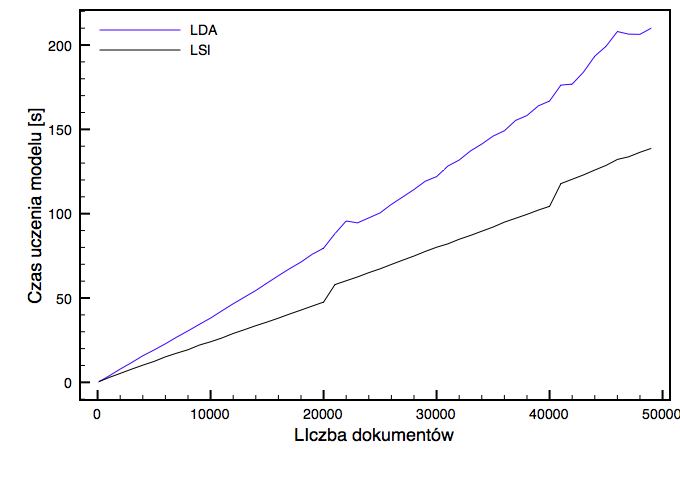
\includegraphics[width=\linewidth]{gfx/time_docs.png}
\caption{Czas uczenia modelu dla 100 tematów}
\label{time-docs}
\end{figure}

\begin{figure}[h]
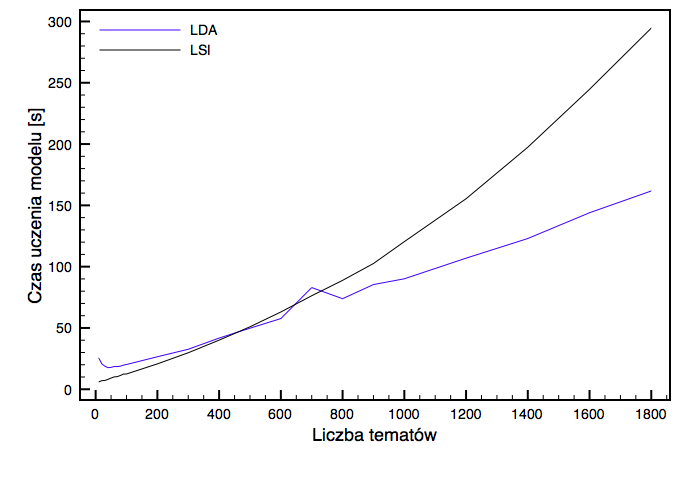
\includegraphics[width=\linewidth]{gfx/time_topics.png}
\caption{Czas uczenia modelu dla 5000 dokumentów}
\label{time-topics}
\end{figure}


\FloatBarrier

\subsection{Metryki z nadzorem}

W tym rozdziale omówiono wyniki otrzymane za pomocą algorytmów LDA i LSI dla
przykładowego problemu opisanego w \ref{sec:example}. Należy zauważyć, że tego
rodzaju ewaluacja wymaga ręcznego przygotowania danych testowych przez
człowieka, co może być nieprakyczne dla dużych zbiorów danych.  Jej zaletą jest
fakt, że mierzy ona faktyczne osiągi danego rozwiązania w rzeczywistych
problemach.

\subsubsection{Ranking dokumentów}

Wykresy \ref{ranks_stemming_comparison} i \ref{ranks_no_stemming_comparison}
przedstawiają sumę kwadratów ranków dokumentów (patrz \ref{sec:ranking}) z
wzorca przygotowanego ręcznie dla danego zapytania w wynikach działania
odpowiednio algorytmów LDA i LSI dla różnej liczby tematów.

Algorytm LDA osiąga ogólnie gorsze wyniki niż LSI, poza przedziałem $50 - 100$
tematów. Gorszy jest też (aczkolwiek niewiele) najlepszy wynik jaki udałoby się
osiągnąć odpowiednio dobierając liczbę tematów. Na wykresie daje się także
zauważyć stochastyczna natura LDA --- podczas gdy dla LSI wyniki niemal
monotonicznie poprawiają się wraz ze wzrostem liczby tematów, dla LDA zdarza się
znaczne pogorszenie wyników przy zwiększeniu tej liczby.

Polepszenie wyników dzięki zastosowaniu stemmingu jest widoczne na pierwszy
rzut oka --- polski jako język silnie fleksyjny jest znakomitym kandydatem do
zastosowania tego typu techniki. W \cite{manning-schuetze} zasugerowano, że ze
stemmingu można zrezygnować dysponując odpowiednio dużym zbiorem danych, jednak
wyniki te uzyskano dla języka angielskiego, którego fleksja jest znacznie mniej
rozbudowana. W tym wypadku zebranie tak dużej ilości danych może być mniej
praktyczne niż skonstruowanie słownika fleksyjnego, takiego jak na przykład ten
opisany w \cite{lubaszewski-slownik}.

Co ciekawe algorytm LDA radzi sobie znacznie lepiej od LSI bez wykorzystania
stemmingu.  Może to być spowodowane trudnością w przypadku LSI połączenia ze
sobą słów, które różnią się formą fleksyjną i są w tym wypadku traktowane
całkowicie osobno.

\begin{figure}[h]
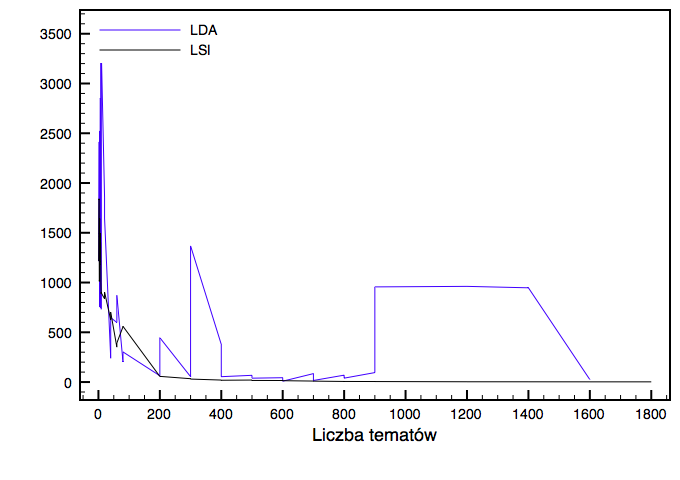
\includegraphics[width=\linewidth]{gfx/ranks_stemming.png}
\caption{Suma kwadratów ranków dokumentów ze wzorca dla testowego zapytania (z wykorzystaniem stemmingu)}
\label{ranks_stemming_comparison}

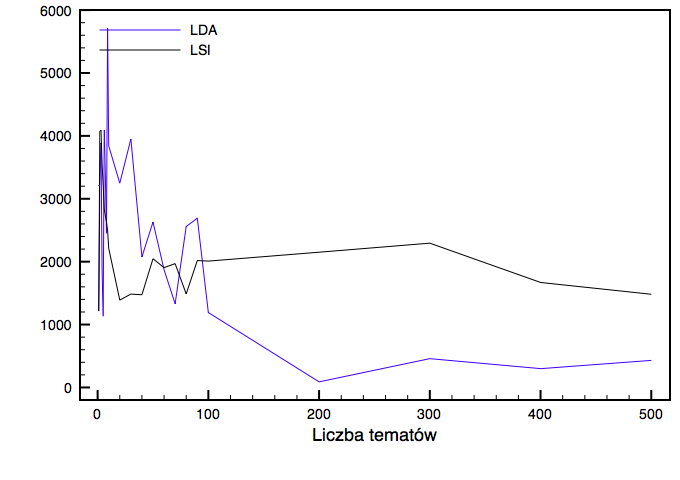
\includegraphics[width=\linewidth]{gfx/ranks_no_stemming.png}
\caption{Suma kwadratów ranków dokumentów ze wzorca dla testowego zapytania (bez wykorzystania stemmingu)}
\label{ranks_no_stemming_comparison}
\end{figure}

\FloatBarrier

\subsubsection{Krzywe ROC}

Krzywe ROC przedstawiają zależność między True Positive Rate --- stosunkiem
liczby poprawnie zwróconych dokumentów do liczby wszystkich skojarzonych
dokumentów, a False Negative Rate --- stosunkiem liczby niepoprawnie zwróconych
dokumentów do liczby wszystkich nieskojarzonych dokumentów:

\begin{equation}
TPR = \frac{TP}{TP + FN}
\end{equation}

\begin{equation}
FPR = \frac{FP}{FP + TN}
\end{equation}

Wykresy \ref{roc_lsi} i \ref{roc_lda} przedstawiają krzywe ROC dla algorytmów
LDA i LSI dla różnych liczb tematów.  Dla dużych liczb tematów algorytm LDA
spisuje się gorzej, jednak można zauważyć, że klasyfikator uzyskany dla 30
tematów jest podobnej jakości lub lepszy jak ten uzyskany przy użyciu LSI dla
100 tematów.


\begin{figure}[h]
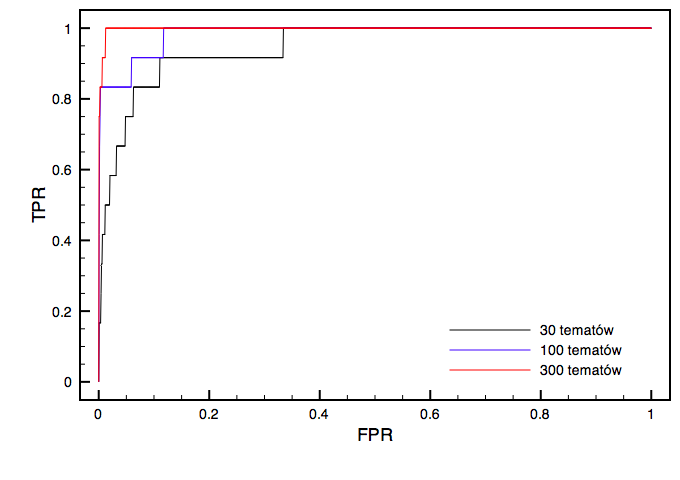
\includegraphics[width=\linewidth]{gfx/lsi_roc.png}
\caption{Krzywe ROC dla algorytmu LSI dla wybranych liczb tematów}
\label{roc_lsi}

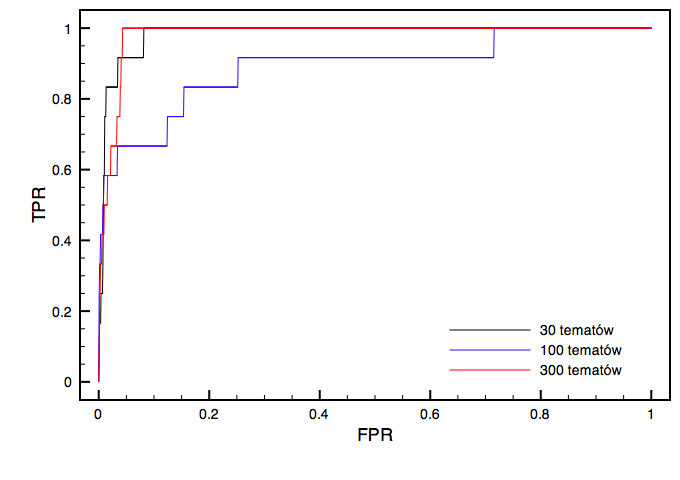
\includegraphics[width=\linewidth]{gfx/lda_roc.png}
\caption{Krzywe ROC dla algorytmu LDA dla wybranych liczb tematów}
\label{roc_lda}
\end{figure}

Na wykresach \ref{roc_lsi_untagged} i \ref{roc_lda_untagged} przedstawione
zostały krzywe ROC dla algorytmów LSI i LDA bez wykorzystania stemmingu.
Ponownie daje się zauważyć lepsze działanie algorytmu LDA w tym wypadku ---
klasyfikator uzyskany dla 300 tematów jest znacznie lepszy od tego uzyskanego
przy pomocy LSI.

\begin{figure}[h]
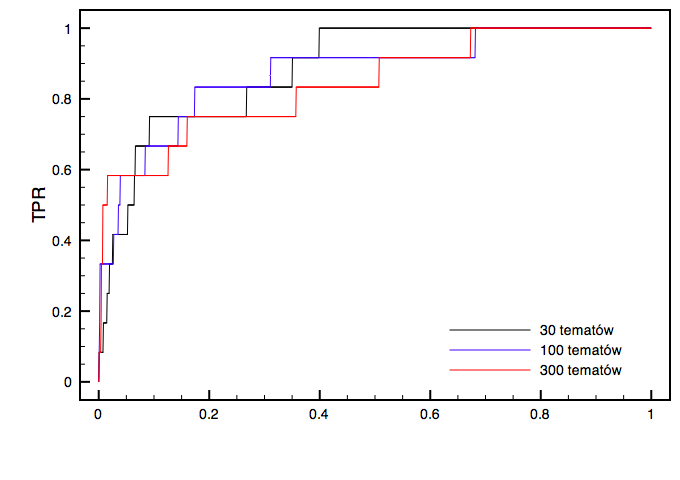
\includegraphics[width=\linewidth]{gfx/lsi_roc_untagged.png}
\caption{Krzywe ROC dla algorytmu LSI dla wybranych liczb tematów bez wykorzystania stemmingu}
\label{roc_lsi_untagged}

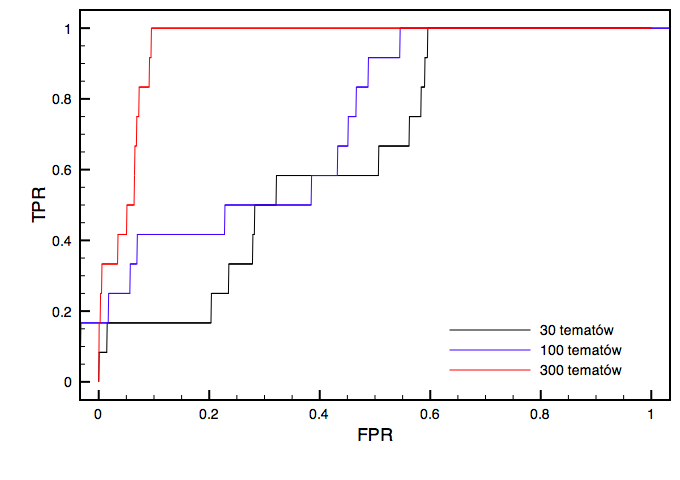
\includegraphics[width=\linewidth]{gfx/lda_roc_untagged.png}
\caption{Krzywe ROC dla algorytmu LDA dla wybranych liczb tematów bez wykorzystania stemmingu}
\label{roc_lda_untagged}
\end{figure}

\FloatBarrier

\subsubsection{Dokładność i kompletność}

Kompletność (stosunek liczby zwróconych skojarzonych dokumentów do liczby
wszystkich skojarzonych dokumentów) i dokładność (stosunek liczby zwróconych
skojarzonych dokumentów do liczby wszystkich zwróconych dokumentów) to częste
metryki w zagadnieniach typu information retrieval. Wybranie jakiegoś poziomu
kompletności reprezentuje pewien kompromis między prawdopodobieństwem zawarcia
wszystkich interesujących wyników w zwróconych danych a częstością
występowania w nich danych skojarzonych, a więc ilością czasu, który musi
poświęcić operator systemu na ich dalsze przetworzenie.

Wykresy \ref{fig:lsi_precision} i \ref{fig:lda_precision} prezentują dokładność
osiąganą przez algorytmy LDA i LSI na różnych poziomach kompletności dla
przykładowego problemu.

Można zauważyć, że LDA daje znacznie gorszą dokładność niż LSI. Nawet najlepiej
dobrana liczba tematów (w tym wypadku 300) pozwala osiągać dokładność
porównywalną jedynie z LSI dla 30 tematów.

\begin{figure}[h]
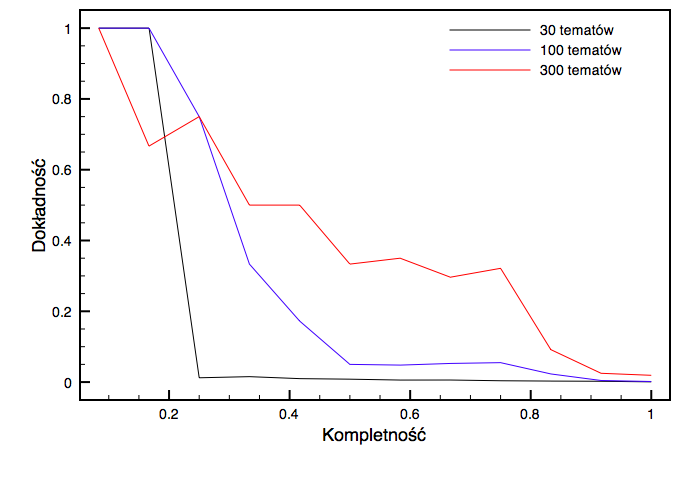
\includegraphics[width=\linewidth]{gfx/lsi_precision.png}
\caption{Dokładność na różnych poziomach kompletności dla algorytmu LSI}
\label{fig:lsi_precision}
\end{figure}

\begin{figure}[h]
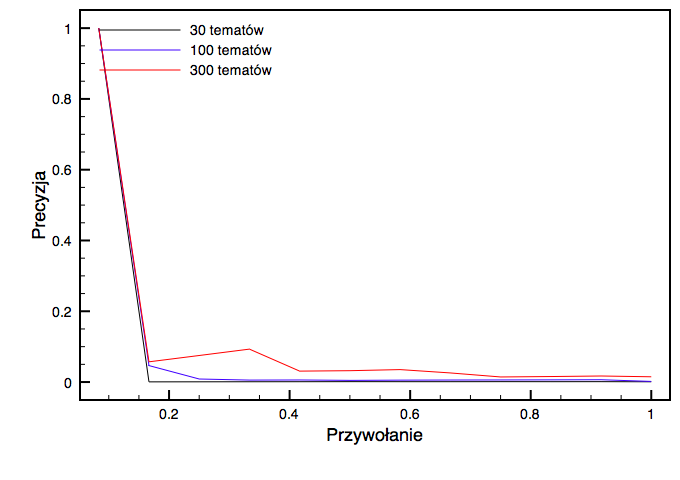
\includegraphics[width=\linewidth]{gfx/lda_precision.png}
\caption{Dokładność na różnych poziomach kompletności dla algorytmu LDA}
\label{fig:lda_precision}
\end{figure}

\FloatBarrier

\subsection{Metryki bez nadzoru (perplexity)}

Współczynnik perplexity, który dla pewnych prawdopodobieństw $p_i$
przypisywanych przez model zdarzeniom obliczyć można zgodnie ze wzorem
\ref{perplexity2}, daje pewne pojęcie o tym, jak dobrze model jest w stanie
przewidzieć nowe dane. Wysokie wartości współczynnika mogą wskazywać, że model
jest przeuczony i będzie słabo uogólniał swoje działania na nieznane dane. Jest
on dobrym wskaźnikiem, jak dobrze model będzie sobie radził z klastrowaniem tego
typu danych.

\begin{equation}
  \label{perplexity2}
  2^{H_i} = \frac{2^{-\sum_{i/1}^n p_ilog_2(p_i)}}{n}
\end{equation}

W tym wypadku $p_i$ to prawdopodobieństwo wygenerowania $i$-tego wyrazu w
kontekście dokumentu, w którym on występuje, czyli pod warunkiem pewnej
kombinacji tematów (która zdaje rozkład prawdopodobieństwa po słowach), jaką
system przyporządkował temu dokumentowi. Liczba $n$ to czynnik normalizujący
będący liczbą wszystkich wyrazów w danym dokumencie.

Wartości współczynnika perplexity dla omawianych metod w zależności od liczby
tematów są przedstawione na wykresie \ref{fig:perplexity}. Wykres demonstruje,
że optymalne wartości współczynnika perplexity zostają osiągnięte w okolicach
50 tematów. W tym wypadku może to sugerować, że mniej więcej na tyle właśnie
grup tematycznych należałoby podzielić ten zbiór danych.

Algorytm LDA zachowuje niski współczynnik perplexity tylko stosunkowo blisko
optymalnej liczby tematów. Takie zachowanie może wymagać dokładnego strojenia
algorytmu do każdego zastosowania, co bywa uciążliwe i czasochłonne.

\begin{figure}[h]
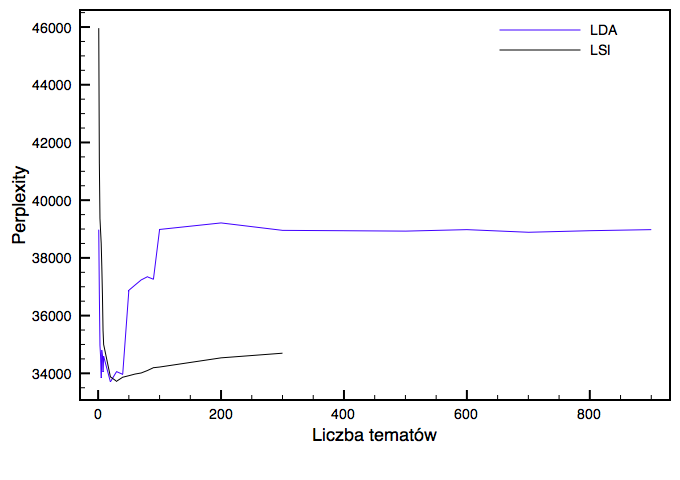
\includegraphics[width=\linewidth]{gfx/perplexity.png}
\caption{Współczynnik perplexity dla LDA i LSI w zależności od liczby tematów}
\label{fig:perplexity}
\end{figure}

\FloatBarrier

\subsection{Wnioski}

Algorytm LDA daje gorszej jakości (a przynajmniej mniej stabilne) wyniki dla
typowych problemów klasyfikacji i wyszukiwania informacji spotykanych w
codziennej praktyce, co nie jest zaskakujące zważywszy na fakt, że LDA można
traktować jako metodę analogiczną do LSI z nałożonym dodatkowym ograniczeniem o
dodatniości wag. Wydaje się za to być w stanie działać w sytuacji, gdy wiele
różnych tokenów oznacza to samo (przypadek bez wykorzystania stemmingu), w
odróżnieniu od LSI, którego wyniki są wtedy całkowicie nieprzydatne. To bardzo
pożądana cecha w przypadku braku odpowiedniego słownika fleksyjnego dla danego
języka.

Metryka perplexity zdaje się sugerować, że LDA jest w stanie uogólniać się na
nieznane dane podobnie dobrze jak LSI, jednak trudniej dobrać parametry, dla
których tak się stanie.

Zarówno LSI jak i LDA skalują się liniowo z liczbą analizowanych dokumentów,
jednak LSI potrzebuje ponadliniowego czasu w zależności od liczby tematów.
Bardzo duże liczby tematów będą praktyczne dopiero dla wielkich korpusów,
jednak jest to kolejne potencjalne zastosowanie dla LDA.

Przewagą LDA wydaje się być jakość generowanych tematów --- przez wymuszenie
dodatnich wag otrzymujemy na najbardziej znaczących pozycjach (z najwyższymi
wagami) słowa opisujące dany dokument/temat, podczas gdy w przypadku LSI mogą
to być słowa najodleg\-lejsze. Takie zachowanie może okazać się korzystne w
zastosowaniach typu tagowanie dokumentów lub automatyczne generowanie
podsumowań czy słów kluczowych, odpowiada ono lepiej postrzeganiu tekstu przez
człowieka, a przecież to on będzie odbiorcą takich podsumowań.

\pagebreak

\section{Podsumowanie}

W tej pracy opisano i poddano porównaniu metody Latent Semantic Indexing i
Latent Dirichlet Analysis pod kątem ich przydatności do automatycznego
porównywania i ekstrahowania tematu dokumentów w języku polskim. W typowych
zadaniach metoda LSI daje lepsze wyniki i łatwiej jest dobrać liczbę tematów
odpowiednią dla danego korpusu. Metoda LDA pozwala ekstrahować tematy lepiej
odpowiadające ludzkiemu postrzeganiu tekstu, przez co lepiej nadaje się do
tagowania czy generowania skrótów dokumentów.

Z braku czasu nie rozważono pewncyh aspektów tego zagadnienia, które mogą być
tematem dalszych badań. Jednym z nich jest wpływ parametrów uczenia modelu LDA
na jakość otrzymywanych wyników. Stosowany tu algorytm
(\cite{gensim-algorithm}) ma trzy takie parametry: $\kappa$ kontrolujący
szybkość zapominania starych informacji, $\gamma_0$ wpływający na zmniejszenie
wagi wczesnych iteracji oraz $S$ oznaczający liczbę dokumentów, które mają być
użyte w każdej iteracji. Można się spodziewać, że dobranie odpowiednich
wartości tych parametrów dla danego problemu znacznie poprawi osiągane wyniki.

Innym potencjalnym kierunkiem rozwoju jest porównanie działania LDA na różnych
rodzajach korpusów. W świetle osiągniętych dobrych wyników dla dużych rozmiarów
słownika można się spodziewać, że korpusy zawierające wiele rzadkich wyrazów,
które są jednak kluczowe dla ich znacznia, takie jak na przykład prace naukowe,
będą dobrze klastrowane przez LDA.

Powiązana z powyższym jest możliwość dalszego porównania działania LDA dla
korpusów w różnych językach. Tutaj również można się spodziewać, że LDA będzie
działać stosunkowo lepiej dla języków o bogatszym słownictwie albo bardziej
rozbudowanej fleksji, zwłaszcze w wypadku braku narzędzi umożliwiających
sprowadzenie tekstu w danym jęzku do form podstawowych.

\label{sec:summary}
\pagebreak

\appendix
\section{Terminy i oznaczenia}
\label{sec:terms}

\begin{itemize}
\item $df_i$ (Document Frequency) --- liczba dokumentów zawierjących $i$-ty token
\item $gf_i$ (Global Frequency) --- stosunek liczby wystąpień $i$-tego tokenu do liczby wszystkich wyrazów w korpusie
\item $tf_i^j$ (Term Frequency) --- stosunek liczby wystąpień $i$-tego tokenu do liczby wszystkich wyrazów w $j$-tym dokumencie
\item Bag-of-words (worek ze słowami) --- założenie o możliowści pominięcia kolejności słów w dokumencie z małą utratą znaczenia
\item Dokument --- tekst lub fragment tekstu
\item FN (False Negatives) --- liczba odrzuconych dokumentów skojarzonych
\item FP (False Positives) --- liczba zwróconych dokumentów skojarzonych
\item Forma podstawowa --- wyróżniona, najprostsza forma wyrazu, przykładowo mianownik rzeczownika
\item Korpus --- zbiór dokumentów
\item LDA --- Latent Dirichlet Allocation
\item LSI --- Latent Semantic Indexing
\item Leksykon --- zbiór wszystkich tokenów występujących w korpusie
\item Polisemia --- możliwość wyrażania różnych koncepcji przez ten sam wyraz, przykładowo zamek
\item Przeuczenie --- zjawisko polegające na zbyt dokładnym odwzorowaniu danych treningowych przez model i utracie zdolności uogólniania
\item SVD --- Singular Value Decomposition
\item Schemat Wagowy --- sposób w jaki dokument jest transformowany do reprezentacji wektorowej
\item Skojarzony --- (o dokumencie) zgodny z kryteriami wyszukiwania, uznany za podobny do dokumentu wzorcowego
\item Słownik --- zbiór wyrazów występująych w korpusie
\item TN (True Negatives) --- liczba odrzuconych dokumentów nieskojarzonych
\item TP (True Positives) --- liczba zwróconych dokumentów skojarzonych
\item Token --- wyraz, znak interpunkcyjny lub grupa znaków traktowana jako całość (na przykład liczba)
\item VSM (Vector Space Model) --- modelowanie języka przez przedstawianie dokumetów jako wektorów
\end{itemize}

\pagebreak

\section{Sposób użycia kodu}
\label{sec:code}

Kod wykorzystany do przeprowadzenia badań w tej pracy znaleźć można pod
\cite{code}. Aby z niego skorzystać konieczne jest zainstalowanie pakietu
gensim. Katalog \emph{bin} zawiera skrypty uruchomieniowe dla przeprowadzonych
eksperymentów. W poniżych poleceniach \emph{model} oznaczna ciąg
\emph{LsiModel} lub ciąg \emph{LdaModel} w zależności od rodzaju modelu, który
ma być testowany. Plik z danymi powinien zawierać dokumenty, każdy w jednej
linii, wyrazy powinny być sprowadzone do form podstawowych, jeżeli takie
rozwiązanie ma być zastosowane.

\begin{itemize}
\item \emph{bin/test\_lsi [plik z korpusem] [model]} --- wypisuje na ekran
listę wygenerowanych tematów
\item \emph{bin/map\_topics [plik z korpusem] [model]} --- oblicza i wypisuje
metrykę $M$ dla różnych liczb tematów
\item \emph{bin/perplexity [plik z korpusem] [model]} --- oblicza i wypisuje
współczynnik perplexity dla różnych liczb tematów
\item \emph{bin/precision [plik z korpusem] [model] [liczba tematów]} ---
oblicza i wypisuje zależność między dokładnością a kompletnością w formie
par [dokładność kompletność] dla zadanej liczby tematów
\item \emph{bin/roc [plik z korpusem] [model] [liczba tematów]} ---
oblicza i wypisuje zależność między TPR a FPR w formie
par [TPR FPR] dla zadanej liczby tematów
\end{itemize}

\pagebreak

\section{Pełna lista tematów}
\label{sec:full-results}

Poniżej zawarto po 10 najbardziej znaczących wyrazów (wraz z ich wagami) dla
wszystkich tematów wygenerowanych przez metody LDA i LSI skonfigurowanych na
100 tematów, dla korpusu notatek PAP.


\begin{table}[h]
\caption{Wszystkie tematy wyekstrahowane przez algorytm LSI}
\begin{tabular}{|c|>{\footnotesize}p{\linewidth}|}
\hline
Lp. & Temat \\\hline

1 & 0.208*procent + 0.160*rok + 0.153*złoty + 0.152*polski + 0.122*spółka + 0.121*milion + 0.111*wzróść + 0.110*punkt + 0.104*akcja + 0.099*powiedzieć\\\hline
2 & -0.275*procent + -0.257*wzróść + -0.252*punkt + -0.213*WIG + -0.189*spaść + -0.182*wynieść + -0.153*sesja + -0.147*akcja + -0.146*złoty + -0.144*spółka\\\hline
3 & 0.477*RATIO + 0.264*mecz + 0.186*pokonać + 0.181*mistrzostwo + 0.146*turniej + 0.117*piłkarski + 0.114*wygrać + 0.111*przegrać + 0.107*świat + 0.107*reprezentacja\\\hline
4 & -0.281*stopień + -0.234*temperatura + -0.224*maksymalny + -0.213*wiatr + -0.208*umiarkowany + -0.202*deszcz + -0.198*słaby + -0.195*opad + 0.194*złoty + -0.170*południe\\\hline
5 & -0.380*złoty + -0.307*grosz + -0.259*dolar + -0.248*euro + 0.200*punkt + -0.197*osiągać + -0.158*milion + 0.148*WIG + -0.148*umocnić + 0.139*procent\\\hline
6 & -0.376*spółka + -0.315*Akcyjna + 0.241*grosz + -0.226*milion + 0.204*zamknięcie + 0.176*euro + 0.168*osiągać + 0.168*punkt + -0.152*bank + 0.143*dolar\\\hline
7 & -0.444*procent + 0.271*spółka + -0.244*rok + 0.205*akcja + -0.186*proca + 0.165*Akcyjna + -0.156*milion + 0.152*giełda + 0.131*zmienić + -0.129*finanse\\\hline
8 & 0.237*sąd + -0.169*RATIO + -0.163*spółka + 0.146*policja + -0.144*Akcyjna + -0.138*unia + -0.137*AWS + 0.135*lato + 0.129*więzienie + 0.126*tysiąc\\\hline
9 & 0.222*europejski + -0.206*AWS + -0.195*sąd + -0.153*procent + 0.151*unia + 0.144*UE + -0.130*wyborczy + -0.120*wybór + 0.119*milion + -0.117*SLD\\\hline
10 & -0.321*RATIO + 0.227*świat + 0.223*mistrzostwo + -0.160*sąd + -0.155*mecz + 0.149*wyścig + 0.131*medal + -0.127*milion + 0.120*miejsce + 0.119*procent\\\hline
11 & 0.292*milion + -0.268*procent + -0.173*cena + 0.140*złoty + -0.130*tonąć + 0.130*bank + 0.130*AWS + -0.122*Akcyjna + 0.122*wartość + 0.116*obligacja\\\hline
12 & -0.316*cena + -0.203*tonąć + -0.161*olej + -0.159*benzyna + -0.155*wzróść + -0.151*napędowy + -0.138*hurtowy + -0.137*turniej + -0.128*nagroda + 0.128*bank\\\hline
13 & -0.241*cena + -0.224*złoty + 0.200*spółka + -0.175*tonąć + -0.157*europejski + 0.157*Akcyjna + -0.156*unia + 0.138*dolar + -0.134*olej + 0.133*procent\\\hline
14 & -0.244*unia + -0.236*europejski + -0.181*turniej + -0.175*nagroda + -0.172*UE + -0.135*numer + -0.135*pula + 0.133*zjednoczony + 0.132*prezydent + 0.130*finanse\\\hline
15 & -0.342*punkt + -0.260*wynieść + -0.187*złoty + 0.183*akcja + -0.177*milion + 0.173*wzróść + 0.169*spadły + -0.157*WIG + 0.156*zmienić + 0.156*papier\\\hline
16 & -0.140*sąd + -0.132*wzróść + -0.131*unia + 0.128*wzrost + 0.123*poziom + -0.120*prezydent + -0.110*państwo + 0.108*spadek + 0.103*stopa + -0.101*sprawa\\\hline
17 & -0.192*finanse + 0.170*milion + 0.149*wzróść + -0.138*turniej + -0.131*ministerstwo + -0.127*stopa + -0.126*wyścig + -0.125*wygrać + 0.124*rok + 0.123*piłkarski\\\hline
18 & 0.239*rok + -0.220*przetarg + -0.163*procent + -0.144*obligacja + -0.142*polski + -0.141*ministerstwo + -0.135*skarb + -0.135*wartość + -0.123*sprzedać + 0.115*netto\\\hline
19 & -0.396*bank + 0.196*minister + 0.173*ustawa + 0.165*finanse + 0.153*ministerstwo + -0.148*stopa + -0.139*procentowy + 0.139*skarb + 0.138*wynieść + 0.128*projekt\\\hline
20 & 0.239*wyścig + 0.212*kolarski + 0.204*etap + -0.201*mistrzostwo + 0.192*grupa + 0.189*wygrać + -0.143*turniej + -0.136*sąd + 0.136*ustawa + 0.129*kilometr\\\hline
\end{tabular}
\end{table}

\begin{table}[h]
\begin{tabular}{|c|>{\footnotesize}p{\linewidth}|}
\hline
Lp. & Temat \\\hline

21 & -0.220*mistrzostwo + -0.213*ustawa + 0.159*wyścig + 0.154*kolarski + 0.147*etap + -0.136*medal + -0.131*świat + -0.119*projekt + 0.116*wygrać + -0.112*sejm\\\hline
22 & 0.259*piłkarski + -0.227*RATIO + 0.200*klub + 0.168*piłkarz + -0.159*złoty + 0.133*dolar + 0.129*poinformować + 0.121*bank + 0.115*trener + 0.113*Daewoo\\\hline
23 & -0.410*bank + -0.205*ustawa + -0.155*rada + 0.148*giełda + 0.130*ministerstwo + 0.128*indeks + -0.128*projekt + -0.127*stopa + -0.119*wynieść + 0.111*poziom\\\hline
24 & -0.329*policja + 0.244*sąd + -0.189*zatrzymać + 0.187*zjednoczony + 0.168*Ameryki + 0.162*stać + 0.158*amerykański + -0.134*mężczyzna + -0.120*policjant + -0.111*rada\\\hline
25 & -0.207*niemiecki + 0.171*ustawa + -0.145*polski + -0.142*koncern + -0.141*mistrzostwo + -0.141*odszkodowanie + -0.141*Daewoo + -0.138*firma + -0.136*motor + -0.130*fundacja\\\hline
26 & 0.243*piłkarski + -0.162*zjednoczony + -0.153*olimpijski + -0.146*Ameryki + -0.144*stać + -0.143*amerykański + 0.134*prezydent + 0.133*reprezentacja + 0.123*Rosja + 0.123*ustawa\\\hline
27 & 0.287*niemiecki + 0.191*odszkodowanie + -0.171*polski + 0.169*fundacja + 0.143*przymusowy + -0.142*dolar + 0.130*liga + 0.127*wypłata + 0.125*puchar + -0.122*grupa\\\hline
28 & 0.244*olimpijski + 0.190*igrzyska + -0.186*zjednoczony + 0.181*rosyjski + 0.174*Rosja + -0.173*stać + -0.166*Ameryki + 0.160*Sydney + -0.159*piłkarski + -0.132*mistrzostwo\\\hline
29 & -0.186*olimpijski + 0.168*Rosja + 0.165*rosyjski + -0.160*rok + -0.150*igrzyska + 0.133*liga + 0.133*proca + -0.117*Sydney + -0.116*papież + -0.114*ii\\\hline
30 & 0.267*olimpijski + 0.210*igrzyska + 0.176*Sydney + 0.142*reprezentacja + -0.140*punkt + 0.137*komitet + -0.134*Dow + -0.129*Jones + -0.125*Nasda + -0.122*premiera\\\hline
31 & 0.243*papież + 0.216*ii + 0.214*Paweł + 0.201*Jan + -0.185*festiwal + -0.164*film + -0.126*międzynarodowy + -0.116*niemiecki + 0.115*skarb + 0.107*kościół\\\hline
32 & -0.233*skarb + 0.199*prezydent + -0.188*proca + 0.182*Kwaśniewski + -0.180*państwo + -0.175*olimpijski + 0.162*zjednoczony + 0.151*Aleksander + 0.151*stać + 0.151*Ameryki\\\hline
33 & -0.257*skarb + -0.218*państwo + -0.148*prezydent + 0.145*bon + -0.143*akcja + 0.140*rentowność + 0.136*spółka + 0.132*proca + 0.131*rada + -0.131*bank\\\hline
34 & 0.195*Daewoo + 0.189*motor + 0.155*koncern + -0.142*zjednoczony + -0.135*olimpijski + -0.132*Ameryki + -0.130*Kwaśniewski + -0.130*minister + -0.126*policja + -0.126*stać\\\hline
35 & -0.235*Daewoo + -0.203*motor + 0.178*miliard + 0.177*dolar + 0.172*niemiecki + 0.149*amerykański + 0.134*deficyt + -0.133*złoty + -0.125*premiera + 0.125*policja\\\hline
36 & -0.201*proca + 0.187*skarb + -0.158*spółka + 0.144*państwo + -0.139*finanse + -0.138*Akcyjna + 0.138*rada + -0.135*deficyt + -0.121*dolar + -0.118*olimpijski\\\hline
37 & -0.207*bank + 0.162*proca + -0.152*rok + 0.147*rada + 0.137*stopa + 0.125*skarb + 0.121*złoty + 0.118*festiwal + -0.118*premiera + -0.114*lato\\\hline
38 & -0.258*Rosja + -0.204*rosyjski + -0.194*AWS + 0.166*Kwaśniewski + 0.141*prezydent + 0.129*Aleksander + 0.116*Jugosławia + -0.111*UW + -0.107*Putin + 0.106*świat\\\hline
39 & -0.196*rada + 0.187*bank + -0.160*Daewoo + -0.147*pieniężny + -0.141*polityka + -0.126*motor + -0.121*stopa + -0.118*procentowy + 0.118*AWS + 0.112*makler\\\hline
40 & -0.400*polski + 0.209*świat + 0.171*film + 0.161*piłkarski + 0.157*premiera + 0.113*bank + 0.113*rząd + 0.097*festiwal + -0.096*liga + -0.095*NATO\\\hline

\end{tabular}
\end{table}

\begin{table}[h]
\begin{tabular}{|c|>{\footnotesize}p{\linewidth}|}
\hline
Lp. & Temat \\\hline

41 & 0.186*lato + 0.167*premiera + -0.129*międzynarodowy + -0.126*Daewoo + 0.121*tysiąc + -0.121*kwartał + -0.120*prokuratura + -0.117*sprawa + 0.111*Buzek + 0.111*rząd\\\hline
42 & -0.220*palestyński + 0.205*rząd + -0.188*izraelski + -0.176*Izrael + -0.158*Palestyńczyk + 0.154*Jugosławia + 0.149*premiera + -0.135*rosyjski + 0.134*Buzek + -0.117*Arafat\\\hline
43 & 0.172*akcja + -0.170*puchar + 0.164*procent + -0.155*miejsce + 0.144*medal + 0.135*mistrzostwo + 0.123*obrót + 0.116*grupa + -0.114*minister + 0.113*zdobyć\\\hline
44 & 0.155*międzynarodowy + -0.140*zostać + -0.138*medal + -0.137*poinformować + 0.135*organizacja + 0.123*świat + -0.119*zdobyć + 0.114*puchar + 0.114*grupa + -0.111*Jugosławia\\\hline
45 & 0.170*tysiąc + -0.162*premiera + 0.154*poinformować + -0.153*rada + 0.146*minister + -0.134*Buzek + 0.125*bank + -0.123*Jerzy + 0.122*finanse + -0.121*puchar\\\hline
46 & -0.252*tysiąc + -0.167*procent + -0.146*puchar + -0.144*akcja + 0.133*wzróść + -0.122*metr + -0.115*dolar + 0.115*mistrzostwo + 0.114*grupa + 0.114*kwartał\\\hline
47 & -0.285*film + -0.211*miliard + -0.147*międzynarodowy + 0.146*warszawa + -0.144*miejsce + 0.124*wystawa + 0.122*minister + -0.119*festiwal + -0.117*zdobyć + -0.111*prezes\\\hline
48 & -0.149*akcja + -0.139*poinformować + 0.114*mistrz + -0.112*miejsce + -0.107*proca + -0.106*Krzaklewski + 0.103*wzróść + 0.101*SLD + 0.101*Kraków + -0.100*pierwsza\\\hline
49 & 0.185*świat + 0.140*rok + -0.132*miliard + -0.121*bank + -0.119*miejsce + -0.111*warszawa + 0.109*polski + -0.106*budżet + -0.105*wzróść + -0.100*pieniądz\\\hline
50 & -0.193*firma + -0.170*nowy + -0.161*Internet + -0.155*internetowy + -0.116*prokuratura + 0.113*Krzaklewski + -0.107*miejsce + 0.106*związek + -0.104*partia + -0.103*wybór\\\hline
51 & 0.207*polski + 0.192*reprezentacja + -0.177*europ + -0.135*organizacja + -0.124*ropa + -0.120*międzynarodowy + -0.120*warszawa + -0.111*minister + -0.110*lato + 0.101*podać\\\hline
52 & -0.308*miliard + -0.202*rok + 0.195*milion + -0.171*tysiąc + 0.155*PKB + 0.152*kwartał + 0.123*wzrost + 0.116*procent + 0.114*ropa + 0.108*netto\\\hline
53 & -0.222*miliard + 0.185*puchar + 0.156*prezes + 0.155*lato + 0.146*poinformować + -0.141*stopa + -0.136*kwartał + -0.126*premiera + -0.125*procentowy + -0.123*wynik\\\hline
54 & 0.200*związek + -0.157*tysiąc + -0.151*film + -0.126*minister + 0.123*prezes + -0.121*miejsce + -0.120*NATO + -0.112*internetowy + -0.111*Internet + -0.111*komitet\\\hline
55 & 0.199*proca + -0.181*miejsce + -0.147*minister + -0.147*reprezentacja + 0.140*mistrz + 0.133*kwartał + -0.128*tysiąc + -0.123*prokuratura + -0.123*sprawa + 0.120*miliard\\\hline
56 & -0.309*miliard + 0.244*milion + -0.141*złoty + -0.125*wystawa + -0.118*firma + 0.117*film + -0.109*AWS + -0.108*puchar + 0.100*praca + -0.097*tysiąc\\\hline
57 & -0.172*poinformować + 0.144*minister + -0.141*puchar + 0.127*mistrz + -0.124*międzynarodowy + -0.117*udział + -0.116*SLD + 0.114*ropa + 0.110*drugi + -0.107*konferencja\\\hline
58 & 0.167*lato + 0.162*kwartał + 0.125*prokuratura + 0.123*miejsce + -0.119*puchar + -0.118*warszawa + 0.116*praca + -0.115*ropa + 0.113*reprezentacja + 0.111*wystawa\\\hline
59 & -0.158*prokuratura + 0.152*tysiąc + 0.128*premiera + -0.122*gdański + 0.122*kwartał + 0.119*ropa + 0.117*publiczny + -0.108*milion + 0.107*narodowy + -0.106*umowa\\\hline
60 & -0.189*puchar + -0.186*minister + 0.157*poinformować + 0.134*miejsce + 0.120*mistrz + 0.118*międzynarodowy + 0.114*wystawa + -0.101*zostać + 0.094*państwo + -0.093*związek\\\hline

\end{tabular}
\end{table}

\begin{table}[h]
\begin{tabular}{|c|>{\footnotesize}p{\linewidth}|}
\hline
Lp. & Temat \\\hline

61 & 0.214*tysiąc + 0.136*rada + -0.133*stopa + -0.128*finanse + 0.121*pierwsza + -0.117*rosyjski + 0.115*bon + -0.115*związek + -0.107*procentowy + -0.103*międzynarodowy\\\hline
62 & -0.159*puchar + 0.158*liga + -0.152*piłkarz + 0.141*minister + 0.130*tysiąc + 0.116*metr + -0.116*wystawa + -0.106*film + 0.096*zagraniczny + 0.096*grupa\\\hline
63 & -0.197*miliard + -0.163*akcja + 0.137*zdobyć + 0.137*medal + 0.136*kwartał + 0.133*dwa + -0.130*polski + -0.124*lato + 0.114*obligacja + 0.113*AWS\\\hline
64 & -0.173*grupa + 0.173*nowy + 0.152*Niemcy + -0.142*dzień + -0.133*ropa + 0.133*międzynarodowy + -0.125*klub + 0.118*komitet + 0.105*amerykański + -0.100*puchar\\\hline
65 & 0.213*rok + 0.211*proca + -0.148*wzróść + -0.148*procent + 0.139*tysiąc + -0.139*lato + -0.137*poinformować + 0.126*miejsce + 0.116*inflacja + 0.113*bon\\\hline
66 & 0.209*piłkarski + -0.137*piłkarz + -0.129*tysiąc + -0.124*wzróść + 0.113*amerykański + 0.112*NATO + -0.106*klub + -0.106*finanse + 0.105*prywatyzacja + 0.101*wynieść\\\hline
67 & -0.172*międzynarodowy + 0.149*grupa + 0.141*europ + 0.124*piłkarz + 0.118*komisja + -0.115*piłkarski + -0.109*runda + 0.097*proca + 0.097*puchar + -0.097*pierwsza\\\hline
68 & 0.177*prezes + 0.138*mistrz + -0.129*podpisać + -0.121*piłkarz + 0.120*prokuratura + -0.119*międzynarodowy + -0.116*komisja + 0.113*grupa + -0.098*koniec + 0.097*firma\\\hline
69 & -0.170*puchar + -0.148*lato + -0.138*akcja + 0.133*prezes + 0.125*nowy + 0.115*budżet + -0.113*wartość + 0.100*PZU + -0.098*pielęgniarka + -0.097*miliard\\\hline
70 & -0.163*nowy + -0.128*amerykański + -0.128*związek + -0.123*prezes + 0.114*dwa + -0.111*unia + -0.110*pielęgniarka + 0.104*komitet + 0.096*wyborczy + -0.094*piłka\\\hline
71 & 0.166*lato + -0.148*reprezentacja + 0.140*międzynarodowy + -0.137*Rosja + -0.127*euro + -0.124*dziecko + 0.123*SLD + 0.122*kosmiczny + 0.112*pierwsza + 0.112*stacja\\\hline
72 & 0.143*nowy + 0.142*akcja + 0.125*lato + -0.117*minister + -0.111*wystawa + 0.111*czerwiec + -0.107*sąd + -0.105*rada + 0.102*prokuratura + -0.100*PZU\\\hline
73 & 0.178*warszawa + -0.149*grupa + 0.118*miliard + -0.112*zostać + -0.111*wartość + 0.110*prasowy + -0.103*euro + 0.102*ropa + -0.100*lipiec + -0.097*dwa\\\hline
74 & 0.186*prokuratura + -0.124*Jugosławia + -0.122*tysiąc + -0.120*AWS + 0.111*premiera + -0.111*gospodarka + -0.106*luty + 0.106*Andrzej + 0.103*rok + -0.102*wicepremier\\\hline
75 & 0.184*europ + -0.184*grupa + -0.157*hokeista + 0.149*koszykarz + -0.147*warszawa + -0.128*new + -0.125*NHL + -0.117*świat + 0.117*międzynarodowy + 0.101*Niemcy\\\hline
76 & 0.153*komisja + 0.130*Ukraina + 0.125*prezes + 0.116*ministerstwo + -0.115*Andrzej + -0.111*film + -0.107*poinformować + 0.103*euro + 0.099*Niemcy + -0.097*PKB\\\hline
77 & -0.179*Ukraina + -0.177*film + -0.148*piłka + -0.129*nożny + 0.127*ministerstwo + 0.124*reprezentacja + 0.114*zostać + -0.103*narodowy + 0.101*platforma + -0.100*Polonia\\\hline
78 & 0.155*mistrz + -0.132*rząd + 0.123*związek + -0.120*koszykarz + -0.100*rok + 0.100*wynieść + -0.099*metr + -0.099*Orlen + -0.092*piłkarski + 0.091*udział\\\hline
79 & 0.156*euro + 0.148*europ + 0.144*czwartek + -0.130*praca + 0.120*piłkarski + -0.119*kwartał + 0.116*środa + 0.112*miejsce + -0.108*tysiąc + -0.108*amerykański\\\hline
80 & 0.177*komisja + 0.154*' + 0.146*mistrz + 0.137*tysiąc + 0.118*prokuratura + -0.113*Niemcy + 0.108*Polska + -0.106*drugi + 0.104*miesiąc + 0.100*dwa\\\hline

\end{tabular}
\end{table}

\begin{table}[h]
\begin{tabular}{|c|>{\footnotesize}p{\linewidth}|}
\hline
Lp. & Temat \\\hline

81 & -0.130*' + -0.118*film + -0.112*Ukraina + 0.106*firma + -0.102*ministerstwo + -0.101*Kraków + 0.099*komisja + -0.097*euro + 0.095*lato + -0.094*Kuczma\\\hline
82 & -0.148*kosmiczny + -0.139*stacja + 0.136*gospodarka + -0.122*grupa + 0.111*choroba + -0.111*badanie + 0.109*nowy + -0.107*centrum + 0.097*wicepremier + 0.096*Janusz\\\hline
83 & -0.141*czerwiec + 0.124*luty + 0.117*styczeń + -0.113*euro + 0.113*wtorek + 0.112*Andrzej + -0.110*maj + 0.104*Ukraina + 0.103*koszykarz + -0.103*sobota\\\hline
84 & -0.152*prezes + 0.134*euro + 0.128*rada + -0.126*dolar amerykański + -0.118*notowanie + 0.118*telewizja + -0.108*klasa + 0.105*SLD + 0.104*piątek + -0.098*osoba\\\hline
85 & 0.154*lato + 0.148*marzec + -0.129*wystawa + 0.116*Ukraina + -0.110*prezes + -0.110*europ + -0.104*samochód + 0.102*warszawa + -0.100*PZU + 0.098*unia\\\hline
86 & -0.181*zostać + -0.162*Ukraina + -0.124*wystawa + 0.123*środa + 0.114*lato + 0.108*runda + 0.107*pierwsza + 0.105*inflacja + 0.103*wartość + 0.103*ostatni\\\hline
87 & -0.168*platforma + 0.139*wtorek + 0.121*PZU + -0.113*obywatelski + -0.106*Orlen + -0.106*środa + -0.105*zostać + -0.104*huta + 0.103*praca + 0.103*wzróść\\\hline
88 & -0.140*zespół + -0.138*komisja + -0.129*lipiec + 0.124*marzec + 0.118*dziecko + 0.117*udział + 0.117*luty + 0.115*wtorek + 0.114*kwiecień + -0.112*Ukraina\\\hline
89 & -0.201*lipiec + -0.161*udział + -0.130*listopad + -0.129*pierwsza + 0.122*Kraków + -0.120*czerwiec + 0.107*zakład + 0.106*czwartek + 0.105*finał + -0.103*sierpień\\\hline
90 & -0.224*styczeń + -0.162*luty + 0.126*lipiec + 0.122*środa + 0.118*film + 0.112*czerwiec + 0.109*listopad + 0.109*rada + -0.109*zostać + 0.107*piątek\\\hline
91 & -0.159*krowa + -0.147*platforma + 0.137*koszykarz + -0.131*styczeń + -0.125*BSE + -0.119*szalony + -0.119*choroba + 0.113*czwartek + 0.112*środa + -0.110*Ukraina\\\hline
92 & 0.165*piątek + 0.159*warszawa + 0.156*budżet + -0.129*Polpharma + -0.125*raca + -0.123*warta + -0.116*środa + -0.115*the + -0.113*czerwiec + -0.108*katamaran\\\hline
93 & 0.137*wtorek + 0.128*film + -0.114*środa + -0.108*połowa + 0.106*Orlen + 0.105*Kraków + -0.103*czwartek + 0.102*rozpocząć + 0.102*piłkarski + -0.101*listopad\\\hline
94 & 0.269*grudzień + 0.218*styczeń + -0.122*czerwiec + 0.121*Czeczenia + 0.118*krowa + 0.111*choroba + 0.110*udział + 0.098*inflacja + -0.096*platforma + 0.094*listopad\\\hline
95 & -0.201*PZU + 0.118*netto + 0.116*maj + -0.116*kosmiczny + -0.115*grudzień + -0.113*Spółka Akcyjna + -0.109*środa + -0.104*styczeń + 0.101*piątek + -0.098*partia\\\hline
96 & 0.154*styczeń + 0.144*Orlen + 0.120*PKN + 0.120*luty + -0.109*nagroda + -0.103*krowa + 0.094*rozpocząć + 0.093*jeden + -0.090*gdański + 0.090*nowy\\\hline
97 & -0.198*styczeń + -0.163*luty + -0.148*nowy + 0.144*jeden + 0.142*koniec + 0.142*listopad + 0.134*firma + -0.119*euro + -0.114*piątek + 0.114*środa\\\hline
98 & -0.187*grudzień + -0.178*PZU + -0.176*listopad + 0.123*luty + -0.121*pierwsza + -0.120*konkurs + -0.106*telewizja + -0.104*zostać + -0.094*miesiąc + -0.094*komitet\\\hline
99 & -0.265*środa + 0.149*inflacja + 0.122*centrum + -0.120*dolar amerykański + 0.113*gmina + -0.113*grupa + -0.110*zostać + -0.093*komitet + -0.091*piłkarz + 0.089*lipiec\\\hline
100 & 0.169*PZU + -0.154*praca + -0.109*osoba + 0.104*listopad + 0.103*ministerstwo + -0.098*Kraków + 0.094*wtorek + 0.091*ostatni + 0.089*notowanie + 0.088*europejski\\\hline
\end{tabular}
\end{table}

\begin{table}[h]
\caption{Wszystkie tematy wyekstrahowane przez algorytm LDA}
\begin{tabular}{|c|>{\footnotesize}p{\linewidth}|}
\hline
Lp. & Temat \\\hline

1 & 0.040*PKB + 0.038*pieniężny + 0.025*polityka + 0.022*deficyt + 0.021*rada + 0.020*procent + 0.019*RPP + 0.018*analityk + 0.014*obrót + 0.014*sport\\\hline
2 & 0.026*prokuratura + 0.019*sąd + 0.018*letni + 0.016*gang + 0.016*oskarżona + 0.016*okręgowy + 0.013*akt + 0.013*oskarżenie + 0.013*efekt + 0.013*przestępstwo\\\hline
3 & 0.025*Bush + 0.020*ii + 0.019*papież + 0.015*Paweł + 0.014*Jan + 0.013*kościół + 0.012*wiek + 0.011*George + 0.011*święty + 0.009*kardynał\\\hline
4 & 0.034*TechWI + 0.027*tour + 0.024*France + 0.022*de + 0.018*sportowy + 0.014*bankowy + 0.014*oszczędność + 0.013*Vivendi + 0.012*bank + 0.010*instancja\\\hline
5 & 0.012*choroba + 0.009*of + 0.008*najnowszy + 0.008*zdrowie + 0.007*lek + 0.007*informować + 0.006*Ameryka + 0.006*naukowy + 0.006*obywatelski + 0.006*numer\\\hline
6 & 0.048*kwartał + 0.027*Laden + 0.026*bin + 0.020*Osama + 0.017*zwierzę + 0.014*zadłużenie + 0.013*transakcja + 0.013*IV + 0.012*tom + 0.012*pies\\\hline
7 & 0.052*spółka + 0.044*skarb + 0.044*Akcyjna + 0.030*akcja + 0.028*Spółka Akcyjna + 0.023*prywatyzacja + 0.023*oferta + 0.020*sprzedaż + 0.020*TP + 0.019*procent\\\hline
8 & 0.032*NBP + 0.026*wczorajszy + 0.020*milion + 0.019*otwierać + 0.016*dolar + 0.016*dekada + 0.015*off + 0.015*podaż + 0.014*play + 0.014*uzgodnić\\\hline
9 & 0.027*huta + 0.020*przejęcie + 0.016*energia + 0.016*belgijski + 0.013*Toruń + 0.012*domniemany + 0.012*gazociąg + 0.012*białostocki + 0.011*rolnik + 0.010*D\\\hline
10 & 0.015*koncert + 0.015*muzyka + 0.010*www + 0.010*podlaski + 0.007*twórca + 0.007*zespół + 0.007*muzyczny + 0.007*festyn + 0.007*proponowany + 0.006*Stefan\\\hline
11 & 0.021*cięcie + 0.016*zaplanować + 0.015*dziesięć + 0.014*przyjść + 0.012*najstarszy + 0.012*siatkarka + 0.012*użycie + 0.011*Śląski + 0.010*światło + 0.010*biały\\\hline
12 & 0.034*netto + 0.032*Daewoo + 0.032*zysk + 0.030*motor + 0.026*milion + 0.023*złoty + 0.018*Jork + 0.017*rok + 0.017*koncern + 0.016*zyskać\\\hline
13 & 0.024*mandat + 0.020*poprawić + 0.017*wykorzystanie + 0.016*kompromis + 0.015*zaginiony + 0.014*pisać + 0.014*ostry + 0.012*Kalisz + 0.012*poczta + 0.010*pogonić\\\hline
14 & 0.030*AZS + 0.022*AWF + 0.015*dymisja + 0.015*Waldemar + 0.014*pokazywać + 0.011*protestujący + 0.011*następca + 0.010*odmawiać + 0.010*zagłada + 0.010*grający\\\hline
15 & 0.016*podejrzany + 0.012*kara + 0.012*Częstochowa + 0.012*małopolski + 0.011*krakowski + 0.011*pozbawienie + 0.010*mózg + 0.010*sala + 0.010*orkiestra + 0.010*koncert\\\hline
16 & 0.015*pilot + 0.012*Artur + 0.011*Albańczyk + 0.011*pojazd + 0.011*Turcja + 0.011*wznowienie + 0.010*analityk + 0.010*wznowić + 0.010*NATO + 0.009*jugosłowiański\\\hline
17 & 0.027*osłabnąć + 0.018*przemysłowy + 0.015*czwartkowy + 0.015*analogiczny + 0.014*telekom + 0.013*zaoferować + 0.013*produkcja + 0.013*klasyczny + 0.012*zremisować + 0.011*styl\\\hline
18 & 0.028*trener + 0.021*sezon + 0.020*klub + 0.019*eliminacja + 0.019*ekstraklasa + 0.018*piłkarski + 0.018*kontrakt + 0.017*Węgier + 0.017*reprezentacja + 0.016*Czech\\\hline
19 & 0.035*Macedonia + 0.015*armia + 0.015*lotniczy + 0.014*lina + 0.014*żołnierz + 0.010*wojsko + 0.010*jednostka + 0.009*dziewięć + 0.008*NATO + 0.008*hotel\\\hline
20 & 0.024*zjednoczony + 0.023*Waszyngton + 0.023*Ameryki + 0.020*amerykan + 0.015*plan + 0.014*stać + 0.014*Iwanow + 0.013*holding + 0.013*ws + 0.011*utworzenie\\\hline

\end{tabular}
\end{table}

\begin{table}[h]
\begin{tabular}{|c|>{\footnotesize}p{\linewidth}|}
\hline
Lp. & Temat \\\hline

21 & 0.018*Miloszevicie + 0.016*Żyd + 0.016*militarny + 0.014*ciężki + 0.013*Przemysław + 0.012*X + 0.011*zdobywca + 0.011*więzień + 0.011*żywy + 0.010*bokser\\\hline
22 & 0.124*wczoraj + 0.041*Orlen + 0.016*możliwy + 0.016*odwołanie + 0.014*akcjonariusz + 0.013*zakończony + 0.012*Optimus + 0.011*obejrzeć + 0.011*sprawozdanie + 0.011*nazwa\\\hline
23 & 0.016*cukier + 0.015*pracownik + 0.015*restrukturyzacja + 0.013*PKP + 0.013*zmniejszenie + 0.012*związkowiec + 0.011*zwolnienie + 0.011*protestować + 0.010*stocznia + 0.010*lubelski\\\hline
24 & 0.023*igrzyska + 0.023*Hiszpan + 0.021*olimpijski + 0.019*trawa + 0.018*długość + 0.018*tenis + 0.017*stołowy + 0.016*włosek + 0.014*gospodarz + 0.014*poszerzenie\\\hline
25 & 0.020*fundacja + 0.018*izba + 0.012*NIK + 0.011*kontrola + 0.011*Rzeszów + 0.010*przekazanie + 0.010*kadencja + 0.009*robotnik + 0.009*wysiłek + 0.008*FSO\\\hline
26 & 0.012*ustawa + 0.012*podatek + 0.011*dochód + 0.008*podatkowy + 0.008*obniżenie + 0.007*ubezpieczenie + 0.007*koszt + 0.007*uzyskany + 0.007*głosowanie + 0.007*zdrowotny\\\hline
27 & 0.019*zainaugurować + 0.016*Zjednoczonych + 0.016*naród + 0.014*pobliże + 0.014*rozwiązać + 0.013*mol + 0.013*Kaczmarek + 0.013*miejscowy + 0.010*student + 0.010*organizacja\\\hline
28 & 0.013*wystartować + 0.013*warta + 0.010*regata + 0.009*Brazylijczyk + 0.009*żużel + 0.009*żużlowy + 0.008*rejs + 0.008*weekend + 0.008*Gustavo + 0.008*terrorystyczny\\\hline
29 & 0.019*podpisanie + 0.018*Japonia + 0.016*lotniczy + 0.015*japoński + 0.015*traktat + 0.013*połączenie + 0.012*Pakistan + 0.012*telekomunikacyjny + 0.011*Pekao + 0.011*międzymiastowa\\\hline
30 & 0.028*nowelizacja + 0.028*ustawa + 0.026*poprawka + 0.024*wydatek + 0.019*sejm + 0.017*senator + 0.016*szkolny + 0.015*IPN + 0.014*powołanie + 0.013*reprezentant\\\hline
31 & 0.028*wrzesień + 0.026*center + 0.021*PZU + 0.020*sierpień + 0.020*towarzystwo + 0.019*terytorium + 0.018*szkoda + 0.016*ubezpieczeniowy + 0.015*zawieszenie + 0.014*Armenia\\\hline
32 & 0.021*skok + 0.017*Dariusz + 0.016*intensywny + 0.015*Rosati + 0.014*konkurs + 0.013*pochmurno + 0.012*północ + 0.012*stolica + 0.011*Małysz + 0.011*Masters\\\hline
33 & 0.038*półrocze + 0.022*negocjacyjny + 0.022*statystyczny + 0.017*kupno + 0.016*skierowany + 0.016*towar + 0.015*produkt + 0.014*Telewizja Polska + 0.014*rolny + 0.013*Kułakowski\\\hline
34 & 0.020*procent + 0.018*proca + 0.013*sondaż + 0.012*wynikać + 0.011*badany + 0.010*senat + 0.010*OBOP + 0.010*respondent + 0.010*faza + 0.010*operator\\\hline
35 & 0.016*komitet + 0.015*Marcin + 0.013*policyjny + 0.013*głos + 0.012*koalicja + 0.012*wyborca + 0.011*nowoczesny + 0.011*Kazimierz + 0.011*Płock + 0.010*poparcie\\\hline
36 & 0.063*euro + 0.054*zamknięcie + 0.044*dolar + 0.034*złoty + 0.034*Kaczyński + 0.031*osiągać + 0.025*umocnić + 0.024*notowanie + 0.020*amerykański + 0.020*porównanie\\\hline
37 & 0.026*Afganistan + 0.026*startować + 0.020*regulacja + 0.020*Słowenia + 0.019*com + 0.016*korzystny + 0.015*dwudniowy + 0.012*miasteczko + 0.012*wykluczać + 0.011*sięgnąć\\\hline
38 & 0.051*zamach + 0.021*Pentagon + 0.016*Kalinowski + 0.014*ludowiec + 0.013*zielony + 0.013*radiowy + 0.011*AIDS + 0.011*Jarosław + 0.011*idea + 0.010*e\\\hline
39 & 0.019*wykonanie + 0.017*wielkopolski + 0.016*gmina + 0.015*woj + 0.014*szachowy + 0.013*wojewoda + 0.012*południowokoreański + 0.012*humanitarny + 0.010*auto + 0.010*rozważać\\\hline

\end{tabular}
\end{table}

\begin{table}[h]
\begin{tabular}{|c|>{\footnotesize}p{\linewidth}|}
\hline
Lp. & Temat \\\hline

40 & 0.021*donosić + 0.021*formuła + 0.016*tor + 0.016*ekipa + 0.016*opozycyjny + 0.014*team + 0.013*Skopje + 0.013*front + 0.012*reprezentować + 0.012*poszukiwany\\\hline
41 & 0.015*wzrost + 0.015*Nasda + 0.015*spadek + 0.014*poniedziałkowy + 0.014*inwestor + 0.014*rynek + 0.012*poziom + 0.010*wczoraj + 0.010*punkt + 0.010*giełda\\\hline
42 & 0.027*Prix + 0.027*granda + 0.015*Australia + 0.015*Rosjanka + 0.014*Edward + 0.013*honorowy + 0.013*świętokrzyski + 0.012*odpaść + 0.011*dowolny + 0.011*objąć\\\hline
43 & 0.020*Kielce + 0.018*szwajcarski + 0.016*mistrzyni + 0.016*rzut + 0.015*pomorski + 0.015*znaczący + 0.013*wygrywać + 0.012*Katarzyna + 0.010*Robert + 0.010*afrykański\\\hline
44 & 0.030*atak + 0.008*Stany Zjednoczone Ameryki + 0.008*Małgorzata + 0.007*zginąć + 0.007*amerykański + 0.007*podać + 0.006*islamski + 0.006*zjednoczony + 0.006*Jordan + 0.006*arabski\\\hline
45 & 0.009*world + 0.008*film + 0.007*zdjęcie + 0.007*Jork + 0.006*afera + 0.006*artystyczny + 0.005*kultura + 0.005*placówka + 0.005*reżyser + 0.005*Czesław\\\hline
46 & 0.011*policja + 0.010*zatrzymać + 0.010*mężczyzna + 0.009*szpital + 0.008*łódzki + 0.007*lekarz + 0.007*forum + 0.007*badanie + 0.006*policjant + 0.006*naukowiec\\\hline
47 & 0.019*niemiecki + 0.016*europejski + 0.016*odszkodowanie + 0.016*UE + 0.016*unia + 0.014*negocjacja + 0.011*Niemcy + 0.010*wypłata + 0.010*pozew + 0.010*unijny\\\hline
48 & 0.046*medal + 0.032*mistrzostwo + 0.026*zdobyć + 0.024*brązowy + 0.021*klasa + 0.020*srebrny + 0.017*odbywać + 0.017*komenda + 0.016*złoty + 0.016*żeglarski\\\hline
49 & 0.040*budżet + 0.034*finanse + 0.016*budżetowy + 0.015*Bydgoszcz + 0.015*deficyt + 0.014*edukacja + 0.012*Jarosław + 0.012*Bauc + 0.012*minister + 0.012*szkoła\\\hline
50 & 0.018*zmniejszyć + 0.016*podpis + 0.014*Poland + 0.014*Nowak + 0.012*oprocentowanie + 0.011*chemiczny + 0.011*weterynaria + 0.011*instytut + 0.011*archiwum + 0.010*taniec\\\hline
51 & 0.049*RATIO + 0.028*mecz + 0.024*turniej + 0.021*pokonać + 0.019*mistrzostwo + 0.018*liga + 0.018*piłkarski + 0.016*finał + 0.016*drużyna + 0.014*polski\\\hline
52 & 0.031*Białoruś + 0.030*białoruski + 0.022*Brazylia + 0.021*Łukaszenka + 0.017*ameryk + 0.017*UC + 0.015*porażka + 0.015*cudzoziemiec + 0.015*Mińsk + 0.015*redukcja\\\hline
53 & 0.052*open + 0.026*FC + 0.025*Barcelona + 0.024*runda + 0.021*Bartosz + 0.017*niekorzystny + 0.016*porto + 0.015*jezioro + 0.014*rozporządzenie + 0.014*doroczny\\\hline
54 & 0.033*Bartoszewski + 0.024*Kuczma + 0.022*handlować + 0.017*Leonid + 0.016*jeździć + 0.016*Rafał + 0.015*upadłość + 0.015*Times + 0.013*podmiot + 0.013*pociąg\\\hline
55 & 0.022*sąd + 0.019*więzienie + 0.014*skazać + 0.014*zabójstwo + 0.012*prokurator + 0.011*okręgowy + 0.011*rejonowy + 0.009*lato + 0.008*grosz + 0.008*Jedwabne\\\hline
56 & 0.026*terroryzm + 0.024*albański + 0.018*Jugosławia + 0.014*Steinhoff + 0.013*wicepremier + 0.011*Janusz + 0.010*bon + 0.010*opozycja + 0.009*prezydent + 0.009*terrorysta\\\hline
57 & 0.027*edycja + 0.023*przejście + 0.021*juniorek + 0.019*graniczny + 0.018*oglądać + 0.016*rezerwa + 0.015*Iwanicki + 0.014*obsługa + 0.014*bandyta + 0.013*oprogramowanie\\\hline
58 & 0.018*serwis + 0.016*aresztować + 0.015*belka + 0.015*konwencja + 0.014*gaza + 0.014*straż + 0.012*apelacyjny + 0.011*list + 0.010*gończy + 0.010*katowicki\\\hline
59 & 0.007*sprawa + 0.007*polski + 0.006*powiedzieć + 0.006*minister + 0.005*sprawiedliwość + 0.005*wszystek + 0.005*stać + 0.005*komitet + 0.005*komisja + 0.005*informacja\\\hline
60 & 0.017*trybunał + 0.015*wojenny + 0.015*zbrodnia + 0.015*porywisty + 0.013*kłopot + 0.012*Haga + 0.012*chorwacki + 0.011*Bośnia + 0.010*Chorwacja + 0.010*wirus\\\hline

\end{tabular}
\end{table}

\begin{table}[h]
\begin{tabular}{|c|>{\footnotesize}p{\linewidth}|}
\hline
Lp. & Temat \\\hline

61 & 0.016*pl + 0.016*nowojorski + 0.014*Internet + 0.012*portal + 0.011*internetowy + 0.010*sieć + 0.010*dużo + 0.009*badanie + 0.009*rok + 0.009*procent\\\hline
62 & 0.041*platforma + 0.034*stopień + 0.029*temperatura + 0.027*wiatr + 0.027*umiarkowany + 0.026*maksymalny + 0.026*słaby + 0.023*opad + 0.021*zachodni + 0.021*południe\\\hline
63 & 0.040*grosz + 0.034*spółka + 0.028*cena + 0.026*Akcyjna + 0.025*obniżyć + 0.023*złoty + 0.021*PKN + 0.021*hurtowy + 0.019*tonąć + 0.017*konsorcjum\\\hline
64 & 0.015*sprzęt + 0.015*hasło + 0.014*słonecznie + 0.014*Sławomir + 0.014*ponieść + 0.014*spadać + 0.013*karny + 0.012*elektroniczny + 0.012*dostępny + 0.012*domowy\\\hline
65 & 0.050*procent + 0.045*punkt + 0.030*wzróść + 0.026*spaść + 0.024*proca + 0.023*WIG + 0.020*giełda + 0.019*złoty + 0.018*milion + 0.017*przetarg\\\hline
66 & 0.033*Wisła + 0.025*rebeliant + 0.021*rozstawić + 0.021*litewski + 0.018*górski + 0.018*Litwa + 0.013*wspólnota + 0.013*współpracować + 0.011*pokonując + 0.011*podtrzymać\\\hline
67 & 0.019*pojednanie + 0.011*Andre + 0.011*ukraiński + 0.010*postęp + 0.010*Agassi + 0.010*przyspieszenie + 0.009*Wenezuela + 0.009*Jałowiecki + 0.009*niezależnie + 0.009*Nature\\\hline
68 & 0.018*policja + 0.016*szczecina + 0.015*sprawca + 0.014*napad + 0.013*miejski + 0.009*Olsztyn + 0.009*ub + 0.009*samochód + 0.009*policjant + 0.008*właściciel\\\hline
69 & 0.028*stopa + 0.028*inflacja + 0.024*procentowy + 0.014*bank + 0.013*łódź + 0.012*centralny + 0.011*spodziewać + 0.011*Ariel + 0.010*szczegół + 0.010*aut\\\hline
70 & 0.027*piłka + 0.024*nożny + 0.017*badacz + 0.015*Polmos + 0.012*Michał + 0.011*cisza + 0.010*PZPN + 0.010*uczcić + 0.010*zwiększać + 0.009*arena\\\hline
71 & 0.022*A + 0.013*Gazprom + 0.013*szwedzki + 0.013*wierny + 0.012*prawomocny + 0.012*uderzyć + 0.011*gazowy + 0.010*dożywotni + 0.010*antydopingowy + 0.010*krzyż\\\hline
72 & 0.020*waluta + 0.016*średnia + 0.015*aukcja + 0.013*zainwestować + 0.013*elektrownia + 0.012*Monika + 0.012*biblioteka + 0.012*Gorzów + 0.011*ekstradycja + 0.010*strefa\\\hline
73 & 0.009*las + 0.007*obserwator + 0.007*muzeum + 0.007*daily + 0.007*tytułem + 0.007*element + 0.007*popularny + 0.007*industries + 0.006*van + 0.006*dokładny\\\hline
74 & 0.016*pomnik + 0.013*Lublin + 0.012*cmentarz + 0.010*pryszczyca + 0.009*pamięć + 0.009*samolot + 0.009*załoga + 0.009*lotnisko + 0.009*ofiara + 0.008*przewoźnik\\\hline
75 & 0.023*powodzić + 0.009*international + 0.008*powódź + 0.008*uczony + 0.008*szefowa + 0.007*szacunek + 0.007*dramat + 0.006*modlitwa + 0.006*udzielenie + 0.006*katedra\\\hline
76 & 0.012*sejm + 0.009*koalicja + 0.008*marszałek + 0.008*talib + 0.008*Maciej + 0.007*prawybory + 0.007*społeczny + 0.007*Afganistan + 0.007*AWS + 0.007*Płażyński\\\hline
77 & 0.042*deszcz + 0.030*ciśnienie + 0.027*hPa + 0.025*wschodni + 0.025*przelotny + 0.021*południowy + 0.020*technologia + 0.019*południowo + 0.018*przejaśnienie + 0.016*powietrze\\\hline
78 & 0.040*ropa + 0.023*naftowy + 0.016*włoski + 0.016*australijski + 0.016*KGHM + 0.015*dostawa + 0.013*mata + 0.012*CCC + 0.012*konsument + 0.012*Londyn\\\hline
79 & 0.039*wyścig + 0.034*kolarski + 0.032*etap + 0.028*wygrać + 0.020*kilometr + 0.019*grupa + 0.016*lider + 0.016*Argentyna + 0.014*kolarz + 0.013*Włoch\\\hline
80 & 0.062*wynieść + 0.034*MIDWIG + 0.030*stracić + 0.020*NI + 0.019*zniżka + 0.016*wicemistrz + 0.015*lipiec + 0.014*juan + 0.014*organizacyjny + 0.014*Grecja\\\hline

\end{tabular}
\end{table}

\begin{table}[h]
\begin{tabular}{|c|>{\footnotesize}p{\linewidth}|}
\hline
Lp. & Temat \\\hline

81 & 0.024*metr + 0.021*rekord + 0.018*lekkoatletyczny + 0.018*bieg + 0.017*szczyt + 0.014*mityng + 0.013*świat + 0.013*ustanowić + 0.012*trasa + 0.012*Korea\\\hline
82 & 0.039*okrąg + 0.027*korupcja + 0.025*Aldona + 0.019*lewica + 0.016*zatwierdzić + 0.015*Norwegia + 0.013*prezentacja + 0.013*ordynacja + 0.011*Egipt + 0.011*KPN\\\hline
83 & 0.012*wyborczy + 0.011*SLD + 0.009*wybór + 0.009*powiedzieć + 0.008*prezydent + 0.007*PSL + 0.007*AWS + 0.006*partia + 0.006*kandydat + 0.006*polityczny\\\hline
84 & 0.036*new + 0.025*łam + 0.022*Edmonton + 0.020*stworzenie + 0.019*York + 0.018*kibic + 0.013*fabryka + 0.011*gra + 0.010*Mariusz + 0.010*sympatyk\\\hline
85 & 0.023*Polka + 0.022*siódmy + 0.016*walc + 0.015*pozycja + 0.013*S + 0.013*sobotni + 0.012*uplasować + 0.012*university + 0.012*tyczka + 0.011*sukces\\\hline
86 & 0.031*zniżkować + 0.026*wywalczyć + 0.017*szczeciński + 0.017*kapitałowy + 0.016*nafta + 0.015*Tomasz + 0.014*poeta + 0.012*zadebiutować + 0.012*zdobywać + 0.012*umożliwić\\\hline
87 & 0.021*Schroeder + 0.017*turecki + 0.016*budowlany + 0.015*Gerhard + 0.015*news + 0.015*królewski + 0.015*uczeń + 0.013*zabytek + 0.011*aktualny + 0.011*zamek\\\hline
88 & 0.030*benzyna + 0.024*napędowy + 0.022*bezrobocie + 0.022*gdański + 0.021*rafineria + 0.018*gram + 0.016*wielkość + 0.015*piętnastka + 0.013*bezrobotny + 0.013*biznesmen\\\hline
89 & 0.065*terrorystyczny + 0.021*prognoza + 0.018*Chiny + 0.016*powodzianin + 0.014*energetyczny + 0.013*Pekin + 0.012*oddać + 0.012*chiński + 0.012*zjednoczony + 0.010*Ameryki\\\hline
90 & 0.015*sztuka + 0.014*wierzyciel + 0.011*wystawa + 0.011*szacować + 0.009*przemyt + 0.009*Donald + 0.007*współczesny + 0.007*from + 0.007*zbiór + 0.007*zabezpieczenie\\\hline
91 & 0.032*film + 0.021*filmowy + 0.017*czeski + 0.016*senat + 0.011*Qua + 0.011*Praga + 0.011*prognozować + 0.011*maraton + 0.010*kino + 0.010*literatura\\\hline
92 & 0.035*siatkarz + 0.028*junior + 0.022*zagrać + 0.019*koszykarka + 0.018*Gdynia + 0.017*Wrocław + 0.016*tabela + 0.015*Estonia + 0.014*Łotwa + 0.014*grać\\\hline
93 & 0.028*kilogram + 0.025*federacja + 0.022*Pomorski + 0.017*FIFA + 0.015*międzynarodowy + 0.011*Sebastian + 0.011*waga + 0.011*koszykówka + 0.010*świat + 0.010*gościć\\\hline
94 & 0.028*general + 0.027*motors + 0.017*tona + 0.014*Corp + 0.014*komórka + 0.013*emerytalny + 0.013*zboże + 0.011*skupić + 0.011*cykl + 0.011*nieprawidłowość\\\hline
95 & 0.023*święto + 0.019*indywidualny + 0.016*przygotowywać + 0.015*Joanna + 0.015*globalny + 0.015*rodzinny + 0.013*boks + 0.013*Carlos + 0.012*gwiazda + 0.012*Arkadiusz\\\hline
96 & 0.027*UEFA + 0.022*zmieniać + 0.019*kasa + 0.016*targ + 0.016*angielski + 0.016*F + 0.012*książka + 0.011*chora + 0.011*uchwalony + 0.011*terytorialny\\\hline
97 & 0.020*Izrael + 0.017*palestyński + 0.016*izraelski + 0.012*Palestyńczyk + 0.008*stacja + 0.008*pokaz + 0.008*typ + 0.008*Arafat + 0.007*szaron + 0.007*los\\\hline
98 & 0.032*tenisista + 0.029*kort + 0.021*rozgrywany + 0.019*strata + 0.018*dziewiąty + 0.017*zakwalifikować + 0.017*Witold + 0.015*wycofać + 0.014*nieznacznie + 0.014*Amerykanin\\\hline
99 & 0.027*festiwal + 0.014*teatr + 0.011*impreza + 0.010*konkurs + 0.010*blok + 0.010*koło + 0.008*nagroda + 0.008*rozpocząć + 0.008*spektakl + 0.007*tegoroczny\\\hline
100 & 0.006*polski + 0.006*porozumienie + 0.006*święta + 0.006*inwestycja + 0.006*skutek + 0.005*przyszły + 0.005*europejski + 0.005*nasz + 0.005*budowa + 0.005*Polska\\\hline

\end{tabular}
\end{table}
\FloatBarrier

\pagebreak

\addcontentsline{toc}{section}{Spis tablic}
\listoftables

\pagebreak
\addcontentsline{toc}{section}{Spis rysunków}
\listoffigures

\pagebreak
\addcontentsline{toc}{section}{Literatura}
\bibliographystyle{abbrv}
\bibliography{thesis}

\enddocument
